\documentclass{UUThesisTemplate}

\usepackage[british]{babel}
\usepackage{hyperref}
\usepackage[autostyle]{csquotes}
\usepackage{booktabs}
\usepackage{tabularx}
% \usepackage{subfiles}
\usepackage{amsmath}
\usepackage{cleveref}
\usepackage{fixme}
\usepackage{enumitem}
\usepackage{graphicx}
\usepackage{afterpage}
\usepackage{type1cm}
% \usepackage[latin1]{inputenc}
% \usepackage[T1]{fontenc}
\usepackage{mathptmx}
\usepackage{amssymb}
\usepackage{siunitx}
\usepackage{subcaption}
\usepackage[titletoc]{appendix}
\usepackage{placeins}

%% Use this to print the dimensions of the text
%% so it can be copied for matplotlib diagrams.
\usepackage{layouts}

%% Use this to show margins
% \usepackage{showframe}


% Vector notation should be bold and italic
\usepackage{bm}
\renewcommand{\vec}{\bm}

\fxsetup{draft,inline,nomargin,theme=color}
\captionsetup[subfigure]{skip=0.333\baselineskip, font=footnotesize}

% The title is never printed but here it is anyway
% \title{Analysis of stereo image in vast repositories of recorded music}

%% Acronyms
\usepackage[automake=immediate]{glossaries-extra}
\setabbreviationstyle[acronym]{long-short}
\makeglossaries{}

% Apparently the only way to prevent all the acronyms from generating spelling errors is to 
% disable ltex on the entire file.
% LTeX: enabled=false

\newabbreviation{ai}{AI}{Artificial Intelligence}
\newabbreviation{ar}{AR}{Augmented Reality}
\newabbreviation{asf}{ASF}{Amplitude Stereo Features}
\newabbreviation{cac}{CAC}{Cut And Clicks}
% \newabbreviation{cd}{CD}{Cochleagram Difference}
\newabbreviation{cd}{CD}{Compact Disc}
\newabbreviation{dft}{DFT}{Discrete Fourier Transform}
\newabbreviation{dirac}{DirAC}{Directional Audio Coding}
\newabbreviation{dl}{DL}{Deep Learning}
\newabbreviation[longplural=Directions of Arrival]{doa}{DOA}{Direction of Arrival}
\newabbreviation{dsp}{DSP}{Digital Signal Processing}
\newabbreviation{erb}{ERB}{Equivalent Rectangular Bandwidth}
\newabbreviation{fa}{FA}{Frequency-Azimuth}
\newabbreviation{faa}{FAA}{Frequency-Azimuth Analysis}
\newabbreviation{fft}{FFT}{Fast Fourier Transform}
\newabbreviation{fir}{FIR}{finite impulse response}
\newabbreviation{fmttm}{FMTTM}{Fly Me To The Moon}
\newabbreviation{genai}{Gen-AI}{Generative Artificial Intelligence}
\newabbreviation{iamf}{IAMF}{Immersive Audio Model and Formats}
\newabbreviation{daw}{DAW}{Digital Audio Workstation}
\newabbreviation{dj}{DJ}{Disc Jockey}

\newabbreviation{rq}{RQ}{research question}

\newabbreviation{iid}{IID}{Interaural Intensity Difference}
\newabbreviation{ipd}{IPD}{Interaural Phase Difference}
\newabbreviation{icpd}{ICPD}{Inter-channel Phase Difference}
\newabbreviation{ccpd}{CCPD}{Cross-channel Phase Difference}
\newabbreviation{ild}{ILD}{Interaural Level Difference}
\newabbreviation{ilr}{ILR}{Interaural Level Ratio}
\newabbreviation{cld}{CLD}{Channel Level Difference}
\newabbreviation{ccad}{CCAD}{Cross-channel Amplitude Difference}
\newabbreviation{icld}{ICLD}{Inter-channel Level Difference}
\newabbreviation{itd}{ITD}{Interaural Time Difference}
\newabbreviation{ictd}{ICTD}{Inter-channel Time Difference}
\newabbreviation{iacc}{IACC}{Interaural Cross Correlation}
\newabbreviation{iccc}{ICCC}{Inter-channel Cross Correlation}
\newabbreviation{icc}{ICC}{Inter-channel Correlation}
\newabbreviation{ic}{IC}{Inter-channel Coherence}
\newabbreviation{iac}{IAC}{Interaural Coherence}
\newabbreviation{itf}{ITF}{Inter-channel Transfer Function}
\newabbreviation{lev}{LEV}{Listener Envelopment}
\newabbreviation{dsd}{DSD}{Directional Loudness Distortion}
\newabbreviation{bms}{BMS}{Bivariate Mixture Space}
\newabbreviation{spl}{SPL}{Sound Pressure Level}
\newabbreviation{iir}{IIR}{Infinite Impulse Response}


\newabbreviation{ishst}{ISHST\textsuperscript{**}}{I Saw Her Standing There\textsuperscript{**}}
\newabbreviation{kks}{KKS}{The Knowledge Foundation}
\newabbreviation{lb}{LB}{Laser Beam}
\newabbreviation{lfe}{LFE}{Low Frequency Effects}
\newabbreviation{llm}{LLM}{Large Language Model}
\newabbreviation{lufs}{LUFS}{Loudness Units Full Scale}
\newabbreviation{mirex}{MIREX}{Music Information Retrieval Evaluation eXchange}
\newabbreviation{mir}{MIR}{Music Information Retrieval}
\newabbreviation{ml}{ML}{Machine Learning}
\newabbreviation{mtg}{MTG}{Music Technology Group}
\newabbreviation{m}{M}{Manifesto}
\newabbreviation{pc}{PC}{Panning Coefficients}
\newabbreviation{ph}{PH}{Panning Histogram}
\newabbreviation{pi}{PI}{Panning Index}
\newabbreviation{picoc}{PICOC}{Population, Intervention, Comparison, Outcome, Context}
\newabbreviation{psf}{PSF}{Phase Stereo Features}
\newabbreviation{qm}{QM}{Qualitative Model}
\newabbreviation{rms}{RMS}{Root Mean Squared}
\newabbreviation{rm}{RM\textsuperscript{*}}{'Round Midnight\textsuperscript{*}} 
\newabbreviation{simpl}{SIMPL}{stereo-input mixed-to-panned level}
\newabbreviation{sip}{SIP}{Stereo Image Profile}
\newabbreviation{slr}{SLR}{Systematic Literature Review}
\newabbreviation{spf}{SPF}{Stereo Panning Features}
\newabbreviation{sps}{SPS}{Stereo Panning Spectrum}
\newabbreviation{ssps}{SSPS}{Spectral Stereo Phase Spread}
\newabbreviation{stft}{STFT}{Short-time Fourier Transform}
\newabbreviation{tf}{TF}{time-frequency}
\newabbreviation{titt}{TITT}{This Is The Thing}
\newabbreviation{vr}{VR}{Virtual Reality}
\newabbreviation{peaq}{PEAQ}{Objective Measurements of Perceived Audio Quality}
\newabbreviation{peaqmc}{PEAQ-MC}{Objective Measurements of Perceived Audio Quality - Multi Channel}
\newabbreviation{cnn}{CNN}{Convolutional Neural Network}

\newabbreviation{ica}{ICA}{Independent Component Analysis}
\newabbreviation{pca}{PCA}{Principal Component Analysis}
\newabbreviation{pqmf}{PQMF}{Pseudo Quadrature Mirror Filter}
\newabbreviation{mpeg}{MPEG}{Moving Picture Experts Group}
\newabbreviation{3gpp}{3GPP}{3rd Generation Partnership Project}

\newabbreviation{asw}{ASW}{Apparent Source Width}
\newabbreviation{fwhm}{FWHM}{Full Width Half Maximum}
\newabbreviation{lef}{LEF}{Lateral Energy Fraction}
\newabbreviation{iqr}{IQR}{Interquartile Range}
\newabbreviation{amt}{AMT}{Auditory Modelling Toolbox}
\newabbreviation{qestral}{QESTRAL}{Quality Evaluation of Spatial Transmission and Reproduction using an Artificial Listener}
\newabbreviation{bcc}{BCC}{Binaural Cue Coding}
\newabbreviation{ps}{PS}{Parametric Stereo}
\newabbreviation{saoc}{SAOC}{Spatial Audio Object Coding}
\newabbreviation{gccphat}{GCC-PHAT}{Generalized Cross Correlation with Phase Transform}
\newabbreviation{mp3}{MP3}{MPEG layer 3}
\newabbreviation{aac}{AAC}{Advanced Audio Coding}
\newabbreviation{ivas}{IVAS}{Immersive Voice and Audio Services}
\newabbreviation{sofa}{SOFA}{Spatially Oriented Format for Acoustics}

\newabbreviation{ir}{IR}{Impulse Response}
\newabbreviation{hrir}{HRIR}{Head-Related Impulse Response}
\newabbreviation{hrtf}{HRTF}{Head-Related Transfer Function}
\newabbreviation{midi}{MIDI}{Musical Instrument Digital Interface}
\newabbreviation{vi}{VI}{Virtual Instrument}
\newabbreviation{mushra}{MUSHRA}{MUlti Stimulus Hidden Reference and Anchor}
\newabbreviation{bsseval}{BSS\_EVAL}{Blind Source Separation Evaluation}
\newabbreviation{psd}{PSS}{Perceptual Spectral Difference}
\newabbreviation{bamq}{BAM-Q}{Binaural-Auditory-Model-based Quality}
\newabbreviation{tff}{TFF}{Time-Frequency Filter}
\newabbreviation{pco}{PCO}{Population, Context, Outcome}
\newabbreviation{wos}{WOS}{Web Of Science}
\newabbreviation{ss}{SS}{Semantic Scholar}
\newabbreviation{cpu}{CPU}{Central Processing Unit}
\newabbreviation{flop}{FLOP}{Floating Point Operation}

\newabbreviation{csv}{CSV}{Comma Separated Variable}
\newabbreviation{tsv}{TSV}{Tab Separated Variable}
\newabbreviation{api}{API}{Application Programming Interface}
\newabbreviation{doi}{DOI}{Digital Object Identifier}
\newabbreviation{url}{URL}{Universal Resource Locator}
\newabbreviation{prisma}{PRISMA}{Preferred Reporting Items for Systematic reviews and Meta-Analyses}
\newabbreviation{adress}{ADRess}{Azimuth Discrimination and Resynthesis}
\newabbreviation{agr}{AGR}{Automatic Genre Recognition}
\newabbreviation{som}{SOM}{Self Organising Map}
\newabbreviation{iresap}{IRESAP}{Information Retrieval in Embedded Systems for Audiovisual Artistic Processes}
\newabbreviation{mdu}{MDU}{Mälardalen Universitet}
\newabbreviation{kmh}{KMH}{Kungliga Musikhögskolan}




% datasets
\newabbreviation{boma}{BOMA}{{Bang \& Olufsen Music for Archimedes}}
\newabbreviation{uiowamis}{UIowaMIS}{University of Iowa Musical Instrument Samples}
% \newabbreviation{}{}{Bach10}
\newabbreviation{btpab}{BTPAB}{ByTeDance paired ambisonic and binaural}
\newabbreviation{dsd100}{DSD100}{Demixing Secret Database}
\newabbreviation{asascbrm}{ASASCBRM}{Database for Automatic Spatial Audio Scene Classification in Binaural Recordings of Music}
\newabbreviation{daoc}{DAOC}{Denon anechoic orchestral collection}
% \newabbreviation{}{}{FAIR-Play}
\newabbreviation{fma}{FMA}{Free Music Archive}
% \newabbreviation{}{}{MedleyDB}
% \newabbreviation{}{}{MedleyDB 2.0}
% \newabbreviation{}{}{MUSDB18}
% \newabbreviation{}{}{MUSDB18-HQ}
\newabbreviation{quasi}{QUASI}{QUaero Audio SIgnals}
\newabbreviation{rwc}{RWC}{Real World Computing}
\newabbreviation{sqam}{SQAM}{EBU Sound Quality Assessment Material}
% \newabbreviation{}{}{Slakh}
\newabbreviation{urmp}{URMP}{University of Rochester Multi-Modal Music Performance}
% \newabbreviation{}{}{ccMixter}
\newabbreviation{arsso}{ARSSO}{Anechoic Recording System for Symphony Orchestra}
\newabbreviation{rioossr}{RIOOSSR}{Recordings of Italian opera orchestra and soloists in a silent room}
\newabbreviation{msss}{MSSS}{Mixing Secrets for The Small Studio}
\newabbreviation{tss}{TSS}{Telefunken Studio Sessions}
\newabbreviation{mtgj}{MTGJ}{Music Technology Group Jamendo}
% \newabbreviation{}{}{Audio and Acoustic Signal Processing Technical Committee Online Resources}
\newabbreviation{maestro}{MAESTRO}{MIDI and Audio Edited for Synchronous TRacks and Organization}
% \newabbreviation{}{}{FiloSax}
% \newabbreviation{}{}{Gamelan Music Dataset}
% \newabbreviation{}{}{mobygratis}


% Journals
\newabbreviation{jaes}{JAES}{Journal of the Audio Engineering Society}
\newabbreviation{eurasip}{EURASIP}{European Association for Signal Processing}


% drawing figures
\usepackage{tikz}
\usetikzlibrary{shapes.geometric}
\usetikzlibrary {arrows.meta}
\usetikzlibrary {arrows}
\usetikzlibrary{positioning}
\usetikzlibrary{fit}
\usetikzlibrary{backgrounds}
\usetikzlibrary{shapes.misc}
\usetikzlibrary{intersections} % name path
\usetikzlibrary{decorations.markings}
\usepackage{pgfplots}
\pgfplotsset{
    compat=1.18,
    table/search path={figures}
}
\usepgfplotslibrary{groupplots}

% Make every plot render to a separate pdf which is included in later runs.
\usepgfplotslibrary{external} 

% Enable this to compile all tikz diagrams separately
% Supposedly it make the compilation faster but it also makes the build directory impossible to navigate
% \tikzexternalize 
% \pgfrealjobname{main}

\graphicspath{{./images_test/}}


%% References
\usepackage[
    bibstyle=ieee,
    citestyle=numeric-comp,
    backend=biber,
    maxcitenames=2,
]{biblatex}
\setcounter{biburlnumpenalty}{9000}
\setcounter{biburlucpenalty}{9000}
\setcounter{biburllcpenalty}{9000}
\addbibresource{../library_biblatex.bib}


% \includeonly{sections/background.tex}

%% Macros
\newcommand{\citeauthorandnumber}[1]{\citeauthor{#1} \cite{#1}}
\newcommand{\q}[1]{\enquote{#1}}
\newcommand{\rqa}{\hyperref[rq:usecase]{$RQ_1$}}
\newcommand{\rqb}{\hyperref[rq:methods]{$RQ_2$}}
\newcommand{\pani}{\enquote{panning index}}
\newcommand{\ambi}{\enquote{ambience index}}

% Edited from UUThesisTemplate.cls
\newcommand{\dedicationLeft}[1]{%
    \cleardoublepage%
    \vspace*{\stretch{3}}%
    \begin{flushleft}%
    {\@dedicationfont\Large\selectfont\emph{#1}}%
    \end{flushleft}%
    \vspace*{\stretch{1}}%
}

%% Custom citation command to print all authors' full names.
\makeatletter
% 1. Create a custom name format that manually grabs the raw, full name strings
\DeclareNameFormat{ieeefullname}{%
  \usebibmacro{name:given-family}
    {\namepartfamily}
    {\namepartgiven} % Safely extracts the complete first name string
    {\namepartprefix}
    {\namepartsuffix}%
  \usebibmacro{name:andothers}%
}

% 2. Link this custom format to your citation macro
\DeclareCiteCommand{\citefullauthors}
  {\usebibmacro{prenote}}
  {%
    % Forces a loop from author 1 to 99, passing them to our custom formatting macro
    \printnames[ieeefullname][1-99]{author}%
  }
  {\multicitedelim}
  {\usebibmacro{postnote}}
\makeatother

%% Custom ciation command to print the publication name
\makeatletter
% Define the citation command wrapper
\DeclareCiteCommand{\citepublication}
  {\usebibmacro{prenote}}
  {%
    % Check if the entry has a journal title (for articles)
    \iffieldundef{journaltitle}
      {% If no journal, check for a book/conference title
       \iffieldundef{booktitle}
         {% Fallback: use main title if it is a book entry
          \printfield[title]{title}}
         {\printfield[booktitle]{booktitle}}}
      {\printfield[journaltitle]{journaltitle}}%
  }
  {\multicitedelim}
  {\usebibmacro{postnote}}
\makeatother



% Numbering of headings down to the subsection level
\numberingdepth{subsection}

% Including headings down to the subsection level in contents
\contentsdepth{subsection}

\tikzset{
    speaker/.pic={
        \draw[black, rotate=-90, transform shape] (-3,0) -- (3,0) -- (2,2) -- (-2,2) -- cycle (-2,2) -- (-2,4) -- (2,4) -- (2,2);
    },
    head/.pic={
        \filldraw[color=black, fill=white] (0,0) circle[radius=1];
        \filldraw[color=black, fill=white] (1.1,0) ellipse (0.1 and 0.2);
        \filldraw[color=black, fill=white] (-1.1,0) ellipse (0.1 and 0.2);
    },
    mic/.pic={
        \filldraw[color=black, fill=white] (0,0) circle[radius=1];
        \draw[color=black, thick] (-1,1) -- (1, 1);
        \draw[color=black] (250:1) -- (250:1 |- 0,-1.618);
        \draw[color=black] (290:1) -- (290:1 |- 0,-1.618);
    },
    flow_input/.style={rounded rectangle, draw=black, minimum height=1cm, minimum width=3cm},
    flow_process/.style={rectangle, draw=black, minimum height=1cm, minimum width=3cm, align=center},
    flow_output/.style={rectangle, rounded corners, draw=black, minimum height=1cm, minimum width=3cm, align=center},
    arrow/.style={->, >=Latex},
    section_label/.style={rectangle, rounded corners, draw=darkgray, fill=lightgray, rotate=90, minimum height=0.618cm, minimum width=4cm},
}

\abstractdummy{
\begin{abstract}
Spatial information is crucial to the listener's experience of music, and stereophonic recordings have long been the standard for capturing this spatiality. Recent advancements in computing, coupled with the availability of new, very large musical corpora, have created opportunities for large-scale quantitative analysis of the stereo image of recorded music. In this licentiate thesis I address a key gap in current research: direct analysis of raw music recordings to describe the stereo image. The work comprises practice-led research, objective experiments, perceptual listening tests, and an extensive literature review. A combination of immersion in the creative aspects of stereo field and thorough mathematical evaluation of the recorded signals created a strong foundation for future research. The studies together revealed that the while there are many existing stereo descriptors, the musical features visible to each one vary considerably and therefore have differing use cases. Moreover, they don't always align with human perception. The combination of research methods was hence a highly effective way to critique the strengths and weakness of objective measurements. Future work should focus on applying and adapting the discovered methods to modern music datasets.
\end{abstract}
}


\captionsetup{font=footnotesize}

\begin{document}
\frontmatter

linewidth in inches: \printinunitsof{in}\prntlen{\linewidth}

linewdith in cm: \printinunitsof{cm}\prntlen{\linewidth}

\listoffixmes
\frontmatterCS

\dedicationLeft{\footnotesize
This thesis is part of the \glsxtrshort{iresap} project - a collaboration between \glsxtrshort{mdu}, \glsxtrshort{kmh}, Spotify, Ericsson, and Teenage Engineering. It was funded by Spotify and \glsxtrshort{kks}.\\Special thanks to Rikard Lindell, Andreas Rossholm, and Elaine Åstrand for their advice and support, and to Wolmar Nyberg Åkerström for donating his \LaTeX~template.
}

\begin{listofpapers}
    \item \fullcite{franklinDevelopmentWebBasedRealTime2025} \label{paper:auxtrument}
    \item \fullcite{miticSystematicLiteratureReview2026}\label{paper:slr}
    \item \fullcite{miticObjectiveComparisonPanning2025}\label{paper:dafx}
    \item \fullcite{miticPerceptualEvaluationBinaurally2026}\label{paper:bth}
\end{listofpapers}

    
\begingroup
    % To adjust the indentation in your table of contents, uncomment and enter the widest numbers for each level
    %  E.g.  \settocnumwidth{widest chapter number}{widest section number}{widest subsection number}...{...}
    %  \settocnumwidth{5}{4}{5}{3}{3}{3}
    \tableofcontents
\endgroup


\mainmatter

\chapter{Introduction}
\label{sec:intro}

It is a widely accepted truth in the world of music production and recording that spatial information in audio is crucial to  listeners' sense of immersion and connection with the music. To capture that spaciousness, stereophonic recording and reproduction has been the standard format since it gained popularity in the 1950s \cite{zagorski-thomasBloomsburyHandbookMusic2020,lanierHIFITWOCHANNELCOMMOTION1957}. The spatial analysis of subsequent decades worth of stereo recordings presents a unique opportunity to study human musicality, as each recording reflects and encodes the creative choices made by the musicians and recordists involved.

Within the music community it is common to speak about spaciousness in a qualitative sense, using terms such as \enquote{stereo image} and \enquote{stereo field} \footnote{The terms \q{stereo image} and \q{stereo field} are freely interchangeable and, as is normal in the music community, I use them both throughout this thesis.} to encompass all audible spatial aspects. In academia however -- and specifically in the \gls{mir} community -- there have been several explicit attempts to translate these discussions into a quantitive domain \cite{tzanetakisStereoPanningFeatures2007,sarroffMeasurementsSpaciousnessStereophonic2008,tardieuProductionEffectAudio2011}. All were performed in an era when musical datasets were \mbox{hand-curated/-labelled}, fairly small (\numrange{1000}{2000} tracks), and, most notably, private. In recent years new musical corpora have become available, e.g. MTG-Jamendo \cite{bogdanovMTGJamendoDatasetAutomatic2019} and \gls{fma} \cite{defferrardFMADatasetMusic2017}, which are both orders of magnitude larger than their predecessors, containing approximately \num{55000} and \num{100000} tracks respectively. In addition, computing techniques in \gls{ml} and \gls{dl} have progressed to the point where it is now possible to learn extremely high-level features on these vast datasets, thereby making sense of the human creativity represented in the recordings. 

A typical use case for spatial descriptors that has emerged both in academia and industry is classification, and in particular, auto-tagging of musical genre/performer \cite{tzanetakisStereoPanningInformation2010,ziemerGoniometersArePowerful2023}. Such features can be used in music similarity and recommendation tasks \cite{gomezMusicSimilaritySystems2008,ziemerNovelRecordingStudio2020}. It has also been shown that stereo field classification of subsections within a larger work can act as a precursor to other tasks such as segmentation, audio enhancement, upmixing, and source separation \cite{barryMusicStructureSegmentation2007,harmaStereoAudioClassification2011,harmaClassificationTimefrequencyRegions2011}. The latter is very relevant to the audio distribution industry, which is currently experimenting with newer audio formats such as ambisonic and object-based audio. While these new formats offer exciting opportunities for both distributors and listeners, there remains a huge back-catalogue of stereophonic recordings that need to remain playable on modern reproduction equipment. A detailed  understanding of their spatial content would therefore be beneficial.

Historically, binaural audio (which is a subclass of stereo) has been of particular interest because its relevance to human hearing. Thus, it is extremely widely studied, and the underlying fundamental techniques are well-established \cite{blauertTechnologyBinauralListening2013}. Yet there remains a gap in current research regarding direct analysis of raw music recordings, and in particular, describing the stereo image of said recordings at a high level. Through the work described in this thesis, I aim to fill that gap. 

I firstly demonstrate use cases where the spatial analysis of stereo audio has the opportunity to solve real-world problems in audio transmission, dissemination, and reproduction. Accordingly, I gather existing objective methods to describe stereo image and assess their abilities to detect the spatial aspects of a variety of musical audio sources.\footnote{Throughout this thesis I use the word \q{objective} quite frequently. The reader is directed to \cref{ch:methodology} for a full discussion of the philosophical implications, but in essence I use the term to infer that the signal processing techniques discussed are deterministic and applicable to any musical recording.} 
\chapter{Research Questions and Contributions}
\label{sec:research_questions_and_contributions}

The underlying purpose of the research documented in this thesis relates to \gls{mir}, and in particular to generating an understanding of the links between human musical creativity and musical output. While it might be possible for the creative people involved to explain how they make their music, it is far more objective to analyse their output as a representation of their musical ideas.

\section{Research Questions}
\label{sec:research_questions}

Given the aforementioned context, the overarching \gls{rq} can be formed as:

\vspace{1em}
\noindent \hspace{4em} \textit{How do music producers use stereo field?}
\vspace{1em}

The basis of the research is access to extremely large musical corpora and modern computing techniques. The number and variety of recordings available for analysis makes them a decent representation of music producers in general. The spatial aspects of each track can be analysed individually using traditional \gls{dsp} techniques and a population-level analysis can be performed on the spatial features of all tracks together. Thus, I have broken down the main \gls{rq} into two smaller ones:

\vspace{1em}
\begin{enumerate}[
    leftmargin=4em,
    rightmargin=4em,
    itemsep=0.618em
]
\item[$RQ_1$:] \textit{How does the stereo image of a recording relate to real-world musical knowledge?} \label{rq:usecase}
\item[$RQ_2$:] \textit{What methods can be used to describe the stereo image of a music recording?} \label{rq:methods}
\end{enumerate}
\vspace{1em}

These concrete questions are addressed through the four papers included in this licentiate thesis. \rqa~provides an important context of what quantitive spatial aspects receive attention from music practitioners, while \rqb~establishes a state-of-the-art baseline of relationships between those quantitive descriptions and objective measurements. The overarching research question spans both licentiate and doctoral studies, with future plans being detailed in \cref{sec:future_work}.


\section{Research contributions}
This section presents a summary of the research contributions achieved by the four included papers and explains their relationship to the \glspl{rq}. Many parts of the research required spatial descriptors to be extracted from raw audio signals. To facilitate this I implemented a library of software tools, allowing all the research tracks to be linked by a common mathematical framework.

\subsection{An understanding of the musical uses of stereo field}
With respect to the overarching research question, the act of personally creating musical output gives an insight into how music producers in general might use stereo field. We initially embarked on such a project, using audio from a remotely-located stereo microphone as the primary sonic material in a set of musical performances. Paper \ref{paper:auxtrument} was a retrospective account of the process, providing technical information to any musicians wishing to make a similar performance in the future. The paper also provided suggestions for future iterations of similar instruments and the standardized \glspl{api} which are built into web browsers, giving a basis for future work.

The software library presented the opportunity to apply a more technical approach to \rqa{}. The exploration of stereo field in existing recordings furthered the knowledge gained from an individual musical project by allowing us to analytically compare stereo fields created by many producers. This allowed us to establish an understanding of the range and variation that stereo field can embody.

\subsection{Signal processing techniques relating to stereo field}
The software implementation and the resulting paper \ref{paper:dafx} contribute an understanding of how some established techniques for measuring stereo field react to existing recorded music. Moreover, that understanding is not limited to the techniques specified in paper \ref{paper:dafx} since I developed the software continuously throughout several literature searches, resulting a full-featured library that includes many other spatial analysis techniques.

In order to fully answer \rqb{}, an extensive \gls{slr} (paper \ref{paper:slr}) was performed with two intentions. First and foremost, the intention was to conclusively find all existing mathematical techniques that describe stereo field. In addition, there was a goal to find \q{cross-pollination} opportunities from disparate areas of audio research which nonetheless derive spatial cues from audio signals. In doing so, it was possible to form a \q{general model} of \glspl{sip}, thereby making it easier to for future researchers to find or create a \gls{sip} that suits their specific use case.

\subsection{Psychoacoustics of mixed music and speech}
The perceptual listening test described in paper \ref{paper:bth} provided a new perspective on a classic problem in psychoacoustics research. While there is extensive literature describing how people perceive music or speech that has been intentionally masked by another sound, our experiment used music and speech that were intended to complement each other. The results firstly suggested that while people prefer speech that is panned towards the centre, there was an opportunity to increase the audible pleasantness by using very subtle panning. Contrary to our initial assumptions, the musical content had far less influence that originally expected, and speech became the dominant audial stream which was paramount to pleasantness for a majority of listeners.

\subsection{Setup for future work on large datasets of audio}
In regard to the future work described in \cref{sec:future_work}, the \gls{slr} provided both a list of relevant audio datasets, and many standardized implementations of mathematical techniques that extract spatial information from audio.
Paper \ref{paper:dafx} also presented a good opportunity to assess the computational complexity of the algorithms implemented in the software library, thereby highlighting some opportunities for optimization when they are applied to extremely large corpora.
\chapter{Background}
\label{ch:background}

% This chapter provides the fundamental background knowledge that underpins the work included in the thesis. 

Music production techniques related to stereo field are thoroughly rooted in the human perception of sounds, exploiting well-understood auditory phenomena for creative means. However, that understanding is a fairly recent development. In fact, musical practice involving stereophonic sound predated the scientific knowledge of perception by several decades, with one of the earliest known examples dating back the late 19th century \cite{munnTelephoneParisOpera1881}. It wasn't until mid 20th century that the work of \citeauthorandnumber{fletcherLoudnessItsDefinition1933} and \citeauthorandnumber{jeffressPlaceTheorySound1948} outlined the psychoacoustic principles that music production would eventually exploit. In this chapter we draw a line from the basic human physiology of the auditory system, through psychoacoustics, \gls{dsp} theory, and music production, eventually linking them all to the modern computing techniques used as the basis for the work detailed in this thesis. 

\section{The mechanics of hearing and auditory perception}
\label{sec:hearing}

The physical characteristics of the human auditory system govern what we as humans are able to perceive. In particular, our perception of frequency, loudness, and directionality are key when assessing stereo field. 

\subsection{Physiology of the inner ear}
\label{sec:inner_ear}

The ear contains three major sections, loosely labelled the \q{outer}, \q{middle}, and \q{inner} ear (see \cref{fig:ear}). When air vibrations (i.e. sound waves) flow into the outer ear, mechanical coupling in the middle ear transmits vibrations to the cochlea -- the major organ of the inner ear. The cochlea is a conical tube which is coiled up into a spiral, filled with an incompressible fluid, and covered on either end by a membrane. Through the centre of the tube runs the basilar membrane, which is a covered in hairs named cilia. When vibrations are mechanically transmitted to the base of the cochlea, the internal fluid responds by transmitting those vibrations to the basilar membrane, and the cilia will bend and twist accordingly. The cilia are linked to nerve fibres, and will initiate electrical pulses when manipulated. These electrical pulses are sent to the brain and interpreted as sounds \cite{lindsayHumanInformationProcessing1972}.

\begin{figure}[htb]
    \centering
    \resizebox{0.5\textwidth}{!}{
        \begin{tikzpicture}
            \node (pic) at (0,0) {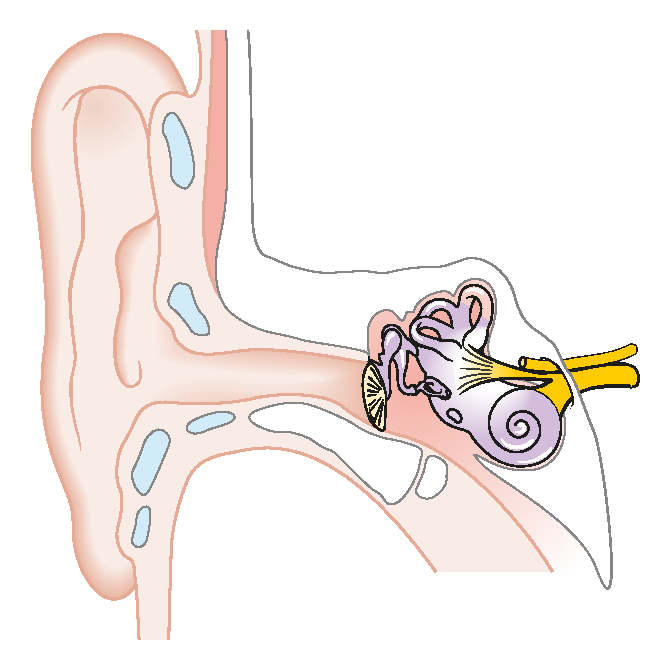
\includegraphics[scale=0.5]{figures/inner_ear.pdf}};
            \node (outer_label) at (-3.5, 0) {Outer ear};
            \node (middle_label) at (0.5, 1.5) {Middle ear};
            \node (inner_label) at (2, 1) {Inner ear};
            \coordinate (outer_point) at (-1.1,-0.4);
            \coordinate (middle_point) at (0.5,-0.1);
            \coordinate (inner_point) at (1.3,-0.5);
            \draw[arrow] (outer_label) -- (outer_point);
            \draw[arrow] (middle_label) -- (middle_point);
            \draw[arrow] (inner_label) -- (inner_point);
        \end{tikzpicture}
    }
    \caption{Diagram of the human ear\textsuperscript{*}. Air flows through the outer ear and vibrates the ear drum. The middle ear mechanically couples the outer ear to the inner ear. The inner ear converts mechanical movements to electrical signals.}
    \label{fig:ear}
    \begin{flushleft}{\scriptsize\textsuperscript{*}\href{https://commons.wikimedia.org/w/index.php?curid=34334173}{Original image} by Cancer Research UK is licensed under \href{https://creativecommons.org/licenses/by-sa/4.0/}{CC BY-SA 4.0}. Annotations have been edited.}\end{flushleft}
\end{figure}

The basilar membrane reacts to a pressure wave from an incoming sound in an elastic way, with a bulge travelling from the base (the widest section) to the apex (the narrowest section). That budge will change amplitude as it travels due to the basilar membrane's non-uniform width and stiffness, and the distance at which is reaches its maximum amplitude depends on the frequency of the incoming sound. Thus, the cilia at different positions along the cochlea have different \q{critical frequencies} that they respond to. The critical frequency increases logarithmically as one moves from the base to the apex, as shown in \cref{fig:cochlea}. The cochlea therefore acts to convert time-domain sound waves into time- and frequency-dependent electrical excitations, enabling us to perceive different frequencies simultaneously. 

\begin{figure}[htb]
    \centering
    \resizebox{\textwidth}{!}{
        
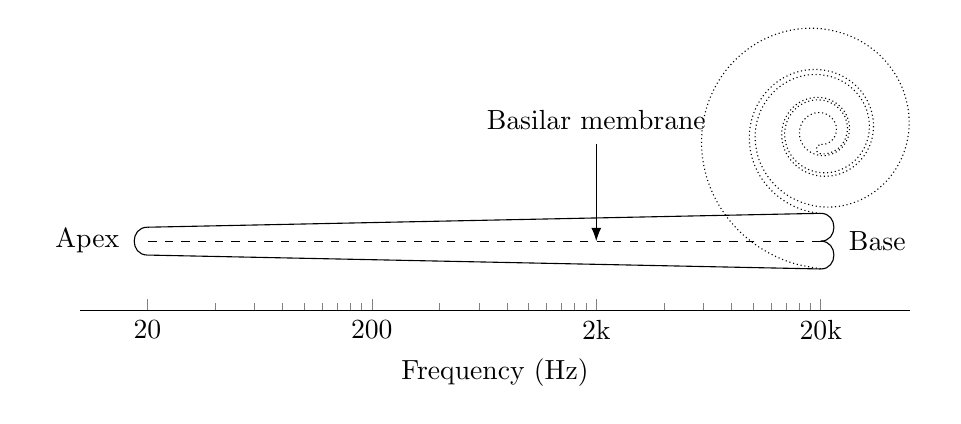
\begin{tikzpicture}
\begin{axis}[
    xmode=log,  
    ymax=2,
    ymin=-0.5,
    xmin=10, 
    xmax=50000, 
    width=\textwidth,
    height=6cm,
    axis x line*=bottom,
    axis y line=none,
    xlabel={Frequency (Hz)},
    xtick={20, 200, 2000, 20000},
    xticklabels={20, 200, 2k, 20k},
]

    \coordinate (base) at (axis cs:20000,0);
    \coordinate (apex) at (axis cs:20,0);
    \coordinate (base_upper) at (axis cs:20000,0.2);
    \coordinate (base_lower) at (axis cs:20000,-0.2);
    \coordinate (apex_upper) at (axis cs:20,0.1);
    \coordinate (apex_lower) at (axis cs:20,-0.1);

    \draw[black] (base_lower) to[bend right=90, looseness=1.618] (base);
    \draw[black] (base) to[bend right=90, looseness=1.618] (base_upper);
    \draw[black] (apex_lower) to[bend left=90, looseness=1.618] (apex_upper);
    \draw[black] (base_upper) -- (apex_upper);
    \draw[black] (base_lower) -- (apex_lower);
    \draw[black, dashed] (base) -- (apex);

    \draw[black,-Latex] (axis cs: 2000, 0.7) node[inner sep=5pt, anchor=south] {Basilar membrane} -- (axis cs: 2000, 0);
\end{axis}

\coordinate (shift) at ($(base) + (0,1.4)$);
\begin{scope}[shift={(shift)}]
\draw[black, densely dotted] plot[smooth, tension=0.618] coordinates {(-0.000,-1.750) (-0.325,-1.688) (-0.627,-1.567) (-0.896,-1.394) (-1.123,-1.178) (-1.302,-0.927) (-1.428,-0.652) (-1.498,-0.363) (-1.512,-0.072) (-1.472,0.212) (-1.380,0.478) (-1.242,0.717) (-1.064,0.922) (-0.855,1.087) (-0.622,1.207) (-0.376,1.280) (-0.125,1.304) (0.122,1.280) (0.356,1.212) (0.568,1.103) (0.753,0.958) (0.904,0.783) (1.018,0.587) (1.090,0.377) (1.122,0.161) (1.112,-0.053) (1.062,-0.258) (0.976,-0.446) (0.859,-0.611) (0.714,-0.749) (0.550,-0.855) (0.371,-0.927) (0.186,-0.963) (-0.000,-0.963) (-0.179,-0.928) (-0.345,-0.862) (-0.493,-0.767) (-0.618,-0.648) (-0.716,-0.510) (-0.786,-0.359) (-0.824,-0.200) (-0.832,-0.040) (-0.810,0.116) (-0.759,0.263) (-0.683,0.394) (-0.586,0.507) (-0.470,0.598) (-0.342,0.664) (-0.207,0.704) (-0.068,0.717) (0.067,0.704) (0.196,0.667) (0.313,0.607) (0.414,0.527) (0.497,0.431) (0.560,0.323) (0.600,0.208) (0.617,0.089) (0.612,-0.029) (0.584,-0.142) (0.537,-0.245) (0.472,-0.336) (0.393,-0.412) (0.302,-0.470) (0.204,-0.510) (0.102,-0.530) (-0.000,-0.530) (-0.098,-0.511) (-0.190,-0.474) (-0.271,-0.422) (-0.340,-0.357) (-0.394,-0.281) (-0.432,-0.197) (-0.453,-0.110) (-0.458,-0.022) (-0.445,0.064) (-0.418,0.145) (-0.376,0.217) (-0.322,0.279) (-0.259,0.329) (-0.188,0.365) (-0.114,0.387) (-0.038,0.395) (0.037,0.388) (0.108,0.367) (0.172,0.334) (0.228,0.290) (0.274,0.237) (0.308,0.178) (0.330,0.114) (0.340,0.049) (0.336,-0.016) (0.321,-0.078) (0.296,-0.135) (0.260,-0.185) (0.216,-0.227) (0.166,-0.259) (0.112,-0.281) (0.056,-0.291) (0.000,-0.291)};
\draw[black, densely dotted] plot[smooth, tension=0.618] coordinates {(-0.000,-1.050) (-0.195,-1.012) (-0.376,-0.940) (-0.537,-0.836) (-0.673,-0.706) (-0.781,-0.556) (-0.856,-0.391) (-0.898,-0.218) (-0.906,-0.043) (-0.881,0.127) (-0.826,0.286) (-0.743,0.429) (-0.637,0.552) (-0.512,0.651) (-0.372,0.722) (-0.225,0.766) (-0.074,0.780) (0.073,0.766) (0.213,0.725) (0.340,0.659) (0.450,0.572) (0.540,0.468) (0.608,0.351) (0.651,0.225) (0.670,0.096) (0.664,-0.032) (0.634,-0.154) (0.583,-0.266) (0.512,-0.365) (0.426,-0.447) (0.328,-0.510) (0.221,-0.553) (0.111,-0.574) (-0.000,-0.574) (-0.107,-0.553) (-0.206,-0.514) (-0.294,-0.457) (-0.368,-0.386) (-0.427,-0.304) (-0.468,-0.214) (-0.491,-0.119) (-0.495,-0.024) (-0.482,0.069) (-0.452,0.156) (-0.406,0.235) (-0.348,0.302) (-0.280,0.356) (-0.204,0.395) (-0.123,0.418) (-0.041,0.426) (0.040,0.419) (0.116,0.396) (0.186,0.360) (0.246,0.313) (0.295,0.256) (0.332,0.192) (0.356,0.123) (0.366,0.053) (0.363,-0.017) (0.347,-0.084) (0.318,-0.145) (0.280,-0.199) (0.233,-0.244) (0.179,-0.279) (0.121,-0.302) (0.060,-0.314) (-0.000,-0.314) (-0.058,-0.302) (-0.112,-0.281) (-0.161,-0.250) (-0.201,-0.211) (-0.233,-0.166) (-0.256,-0.117) (-0.268,-0.065) (-0.271,-0.013) (-0.263,0.038) (-0.247,0.085) (-0.222,0.128) (-0.190,0.165) (-0.153,0.194) (-0.111,0.216) (-0.067,0.229) (-0.022,0.233) (0.022,0.229) (0.064,0.216) (0.101,0.197) (0.134,0.171) (0.161,0.140) (0.182,0.105) (0.195,0.067) (0.200,0.029) (0.198,-0.009) (0.189,-0.046) (0.174,-0.079) (0.153,-0.109) (0.127,-0.133) (0.098,-0.152) (0.066,-0.165) (0.033,-0.171) (0.000,-0.171)};
\draw[black, densely dotted] (0.000,-0.291) to[bend left=90, looseness=1.618] (0.000,-0.171);
\end{scope}

\node[black] at (base) [inner sep=10pt, anchor=west] {Base};
\node[black] at (apex) [inner sep=10pt, anchor=east] {Apex};

\end{tikzpicture}

    }
    \caption{Tonotopic diagram of the human cochlea. Dotted lines represent the cochlea in its normal shape while solid lines show a hypothetical unfurled cochlea with the basilar membrane running down the centre shown as a dashed line. The frequency response of the basilar membrane changes logarithmically along its length, with high frequencies detected at the base and low frequencies at the apex. }
    \label{fig:cochlea}
\end{figure}

\subsection{Directional hearing}
\label{sec:directional_hearing}
\Cref{sec:inner_ear} explains how sound waves are translated in to electrical impulses inside a single ear. When this mechanism is expanded to both ears, combinations of the two sets of electrical impulses can be combined to determine the direction of an incoming sound. 

The psychoacoustic study of spatial hearing has been an active area of research since the mid 20th century, with early examples including the Jeffress model in which time differences between sound events at each ear contribute to a person's ability to locate sounds in space \cite{jeffressPlaceTheorySound1948}. The work of \citeauthor{lindemannEvaluationInterauralSignal1982} a few decades later expanded on this idea by translating the earlier theory to a \gls{dsp} context, and establishing the \gls{ild}, \gls{itd}, and \gls{iacc} as important measures to describe the spatial aspects of binaural signals in a quantifiable way \cite{lindemannEvaluationInterauralSignal1982}.


\begin{figure}[htb]
    \centering
    \resizebox{\textwidth}{!}{
        \begin{tikzpicture}
        \pgfmathsetmacro{\pibyfour}{0.7853981634}
        \pgfmathsetmacro{\ildamp}{0.18}

            % ILD speaker
            \begin{scope}[rotate around={30:(0,0)}]
                \coordinate (speaker_loc) at (4,0);
                \pic[transform shape, scale=0.2] (itd_speaker) at (speaker_loc) {speaker};
                \draw[decorate, decoration={expanding waves, angle=28,segment length=0.4cm}] (speaker_loc) -- (-2,0);
                % \draw[black] (4,0) -- (-4,0);
                \coordinate (shadow_top) at (0,1);
                \coordinate (shadow_middle) at (-2,0);
                \coordinate (shadow_bottom) at (0,-1);
            \end{scope}

            % ILD head
            \fill[lightgray] plot [smooth, tension=1.618] coordinates {(shadow_top) (shadow_middle) (shadow_bottom)};
            \pic[transform shape] (itd_head) at (0,0) {head};
            \node[section_label, minimum width=5.5cm] (itd_label) at (-3, 0) {\glsxtrshort{ild}};

            \begin{scope}[xshift=6cm, yshift=-2cm]
                \begin{axis}[
                    height=6cm, 
                    width=10cm, 
                    ymax=1,
                    ymin=-1,
                    xmin=-1,
                    xmax=11,
                    axis x line=center,
                    axis y line=none,
                    ticks=none,
                    xlabel={time},
                    xlabel style=below right,
                ]
                \addplot[domain=0:10, no markers, smooth] file {generated/ild_L.dat};
                \addplot[domain=0:10, no markers, smooth] file {generated/ild_R.dat};
                \addplot[densely dotted] coordinates {(0, 0.5+\ildamp) (10, 0.5+\ildamp)};
                \addplot[densely dotted] coordinates {(0, 0.5-\ildamp) (10, 0.5-\ildamp)};
                \addplot[densely dotted] coordinates {(0, -0.5+\ildamp*2) (10, -0.5+\ildamp*2)};
                \addplot[densely dotted] coordinates {(0, -0.5-\ildamp*2) (10, -0.5-\ildamp*2)};
                \addplot[latex-latex] coordinates {(-0.2, 0.5+\ildamp) (-0.2, 0.5-\ildamp)};
                \addplot[latex-latex] coordinates {(-0.2, -0.5+\ildamp*2) (-0.2, -0.5-\ildamp*2)};
                \node (a1) at (axis cs: -0.5, 0.5) {$a_L$};
                \node (a2) at (axis cs: -0.5, -0.5) {$a_R$};
                \coordinate (ild_left_y) at (yticklabel cs: 0.75);
                \coordinate (ild_right_y) at (yticklabel cs: 0.25);
                \end{axis}
            \end{scope}

            \node[anchor=east] at (ild_left_y) {Left};
            \node[anchor=east] at (ild_right_y) {Right};


            % ITD 
            \begin{scope}[yshift=-6cm]
                % ITD speaker
                \begin{scope}[rotate around={30:(0,0)}]
                    \coordinate (speaker_loc) at (4,0);
                    \pic[transform shape, scale=0.2] (itd_speaker) at (speaker_loc) {speaker};
                \end{scope}

                % ILD head
                \pic[transform shape] (ild_head) at (0,0) {head};
                \coordinate (left_ear) at (-1.1,0);
                \coordinate (right_ear) at (1.1,0);
                \draw[-Stealth] (speaker_loc) -- (left_ear) node[midway, above] {$d_L$};
                \draw[-Stealth] (speaker_loc) -- (right_ear) node[midway, below] {$d_R$};
                % \node[right] at (4,0) {$d_L > d_R$};
                \node[section_label, minimum width=5.5cm] (itd_label) at (-3, 0) {\glsxtrshort{itd}};

                \begin{scope}[xshift=6cm,yshift=-2cm]
                    \begin{axis}[
                        height=6cm, 
                        width=10cm, 
                        ymax=1.5,
                        ymin=-1,
                        xmin=-1,
                        xmax=11,
                        axis x line=center,
                        axis y line=none,
                        ticks=none,
                        xlabel={time},
                        xlabel style=below right,
                    ]
                    \addplot[domain=0:10, no markers, smooth] file {generated/itd_L.dat};
                    \addplot[domain=0:10, no markers, smooth] file {generated/itd_R.dat};
                    \addplot[densely dotted] coordinates {(\pibyfour 4, 1) (\pibyfour, -1)};
                    \addplot[densely dotted] coordinates {(\pibyfour + 1, 1) (\pibyfour + 1, -1)};
                    \node (tr) at (axis cs: \pibyfour,1.1) {$t_r$};
                    \node (tl) at (axis cs: \pibyfour+1,1.1) {$t_l$};
                    \coordinate (itd_left_y) at (yticklabel cs: 0.6);
                    \coordinate (itd_right_y) at (yticklabel cs: 0.2);
                    \end{axis}
                \end{scope}

                \node[anchor=east] at (itd_left_y) {Left};
                \node[anchor=east] at (itd_right_y) {Right};

            \end{scope}

        \end{tikzpicture}
    }
    \caption{Illustration of how humans perceive the direction of an incoming sound. The physical barrier of the head causes an \glsxtrfull{ild} between sound waves received at the two ears ($a_R-a_L$). The difference in distance from the source to the ears ($d_R - d_L$) causes an \glsxtrfull{itd} between the two ears ($t_l-t_r$).}
    \label{fig:directional_hearing}
\end{figure}

Put simply, we are able to perceive the incoming direction of a sound by observing both the amplitude difference and time difference of coincident sound waves arriving at the left and right ears. Figure \cref{fig:directional_hearing} shows how these two properties enable directional hearing. Firstly, the head itself creates a physical barrier that attenuates sound waves at one ear more-so that at the other ear. Secondly, the difference in distance between the sound source and each ear will create a time delay between the received signals. Over time we learn to associate patterns in \gls{itd}/\gls{ild} with the physical location of the sound source.

The relative importance of \gls{ild} and \gls{itd} differ depending on the frequency of the incoming sound. The reasons for this are twofold. Firstly, a person's inter-aural distance (the physical distance between their ears) must be longer than the wavelength of the incoming sound wave in order for them to detect the phase difference between wave peaks. In this case, it is often referred to as \gls{ipd}, which accounts for the centre frequency of the critical band. Secondly the cilia that line the basilar membrane inside the cochlea can only detect the fine structure of a sound wave up until roughly \qty{1.6}{\kHz} \cite{lindemannEvaluationInterauralSignal1982}. \citeauthor{lindemannEvaluationInterauralSignal1982} gives a rule of thumb that time differences of less than \qty{7.5}{\ms} are heard as a single auditory event (for which direction could be inferred), and differences above \qty{21}{\ms} are heard as uncorrelated events \cite{lindemannEvaluationInterauralSignal1982}. Hence, at \qty{1.6}{\kHz} and below \gls{itd} is more important, whereas above \qty{1.6}{\kHz} \gls{ild} is more important. Furthermore, \citeauthor{blauertSpatialHearingOne1996}'s subsequent work found firstly that both \gls{ild} and \gls{itd} are relevant within the frequency band surrounding \qty{1.6}{\kHz}, and secondly that the angle of incidence of the sound wave plays a role in how the cues are perceived \cite{blauertSpatialHearingOne1996}. Despite this, Lindemann's rules of thumb are still broadly accepted, even being encoded into international standards such as \citetitle{iso-11172-3:mpeg_audio} \cite{iso-11172-3:mpeg_audio}. As an example, \cref{fig:example_pan} shows two recordings (a high-frequency hi-hat and a low-frequency kick drum) that originate from the right-hand side of a listener. The high-frequency hi-hat has a large \gls{ild} and ambiguous \gls{ipd}, whereas the low-frequency kick drum has negligible \gls{ild}, but an interpretable \gls{ipd}.


\begin{figure}[htb]
    \centering
    \includegraphics[scale=0.96]{hihat_kick.pdf}
    \caption{Example sounds coming from the right-hand side, recorded binaurally. High-frequency content (above) has a large \gls{ild} and ambiguous \gls{ipd}, whereas low-frequency content (below) has negligible \gls{ild}, but an interpretable \gls{ipd}.}
    \label{fig:example_pan}
\end{figure}

\subsection{Loudness perception}
While we have established that the \gls{ild} is a key factor of directional hearing, a more detailed understanding of the link between perceived loudness and sound wave intensity is necessary for musical applications.

We perceive the loudness of sound, not in terms of the absolute amplitude of the sound wave, but the \textit{power} of the sound wave. Mathematically speaking, perceived loudness is proportional to the \gls{rms} \gls{spl} raised to an exponent \cite{mooreIntroductionPsychologyHearing2013}. Observing that the calculation of \gls{rms} naturally involves taking the square of the original time function (see \cref{eq:rms_cont,eq:rms_disc} for the continuous and discrete forms respectively), it follows that multiplication of a signal by $\sqrt{2}$ will result in double perceived loudness. Conversely, multiplying a signal by $\frac{1}{\sqrt{2}}$ will halve the perceived loudness.

\begin{align}
    f_{RMS}(t) &= \sqrt{\frac{1}{T_2 - T_1} \int_{T_1}^{T_2}[f(t)^2]dt} \label{eq:rms_cont}\\
    f_{RMS}[n] &= \sqrt{\frac{1}{N}\sum_{n=0}^{N}f[n]^2} \label{eq:rms_disc}
\end{align}

This basic rule is relevant when two sounds are mixed in music production. It defines a precise, mathematical relationship between perceived loudness and the amplification applied by the production equipment or software.

\section{Music production}
\label{sec:music_production}

The principles of our auditory perception have been exploited for creative use since the turn of the 20th century. Early stereophony came from the world of cinema, with sound technicians adding multiple speakers to enable spatial effects\footnote{A typical use case was to match the origin of a voice with the actor's location on the screen.}. Eventually migrating into the music industry, stereophonic recording became the norm in the 1950s \cite{lanierHIFITWOCHANNELCOMMOTION1957,izhakiPanning2023,AbbeyRoadOurStory}. While both cinema and music practitioners have long known that using two speakers for reproduction enabled spatial effects, knowledge of how to \textit{control} those effects came with the psychoacoustic understanding detailed in \cref{sec:hearing}. 


\subsection{Panning}
\label{sec:panning}
The concepts of directional hearing are applied in music production to make sound sources appear as though they originate from a specific direction or position, often referred to as the \q{phantom position}. In recording studio vernacular, this is call \q{panning}. In accordance with the two signal differences a that humans are able to detect (\gls{ild} and \gls{itd}), there are also two basic types of panning -- amplitude panning and time panning. By way of example, \cref{fig:phantom_amplitude} shows how the phantom position can be moved anywhere in between the speakers that are reproducing the sound by applying different amplitude gains to the left and right channel of a stereo recording.

\begin{figure}[htb]
    \centering

    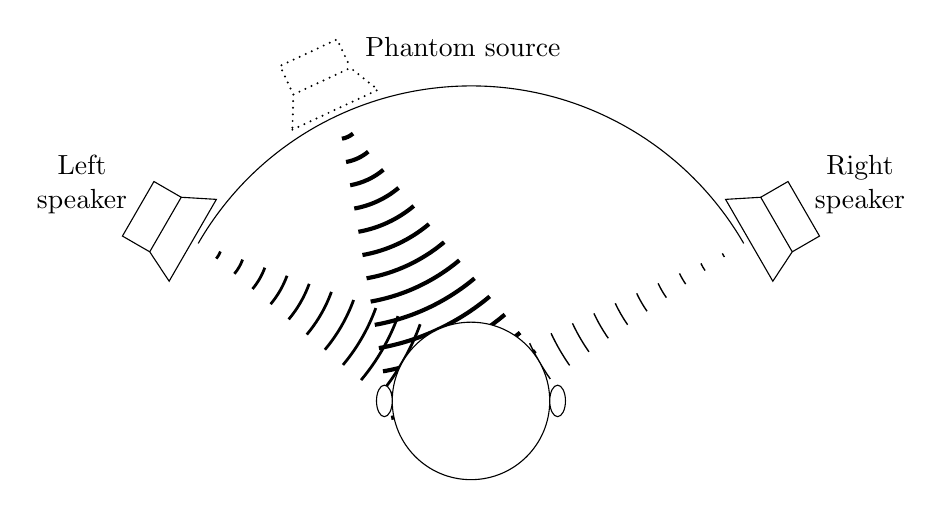
\begin{tikzpicture}
        \def\rad{4};
        \def\expand{1.02};
        \def\soundwaveangle{10};
        \def\soundwavesegmentlength{0.3cm};

        \begin{scope}[rotate around={150:(0,0)}]
            \pic[transform shape, scale=0.2] (left_speaker) at (\rad*\expand,0) {speaker};
        \end{scope}

        \begin{scope}[rotate around={30:(0,0)}]
            \pic[transform shape, scale=0.2] (right_speaker) at (\rad*\expand,0) {speaker};
        \end{scope}
        
        \begin{scope}[rotate around={115:(0,0)}]
            \pic[transform shape, scale=0.2, dotted, line width=0.8pt, line cap=round, dash pattern=on 0pt off 3\pgflinewidth] (phantom_speaker) at (\rad*\expand,0) {speaker};
        \end{scope}

        % labels
        \node[anchor=base east, align=center] (left_label) at (150:\rad+0.9) {Left\\speaker};
        \node[anchor=base west, align=center] (right_label) at (30:\rad+0.9) {Right\\speaker};
        \node[anchor=south west, align=center] (right_label) at (109:\rad+0.5) {Phantom source};

        % Stereo image
        \draw[decorate, decoration={expanding waves, angle=15, segment length=\soundwavesegmentlength}, line width=1.5pt] (115:\rad) -- (0,0);
        \draw[decorate, decoration={expanding waves, angle=10, segment length=\soundwavesegmentlength}, line width=1pt] (150:\rad) -- (0,0);
        \draw[decorate, decoration={expanding waves, angle=5, segment length=\soundwavesegmentlength}, line width=0.5pt] (30:\rad) -- (0,0);

        % Draw full stereo image arc
        \draw (150:\rad) arc (150:30:\rad);

        % Music producer
        \pic (producer) at (0,0) {head};

    \end{tikzpicture}
    \caption{Perception of a phantom sound source created by amplitude panning. The sound wave from the left speaker has higher amplitude than that of the right speaker, thereby creating a phantom source which appears to come from the left.}
    \label{fig:phantom_amplitude}
\end{figure}

Time panning (otherwise known as the \q{Haas effect}) exploits the phenomenon that the first ear to hear a sound generally dictates the direction that it appeared to come from. The process is to simply delay the signal in one channel by a time value within the \q{Haas window} (typically less than 40ms). The undelayed channel will then dictate the phantom direction of the original source. In music production it is used both for panning and to add spaciousness to a recording \cite{stewartWhatHaasEffect2022,izhakiPanning2023}. 

Another frequently used technique is \q{binaural panning}, which assigns combinations of amplitude and time difference to each stereo channel. This is typically achieved by using a \gls{hrir}. An \gls{hrir} is a pair of impulse responses recorded with microphones placed in the ears of either a real person or a dummy head. To obtain an \gls{hrir}, a known excitation signal is played from a specific position in a room and recorded with said binaural microphones (see \cref{fig:phantom_binaural}). The \gls{hrir} can then be convolved with any other monophonic recording to make it appear as though the recording came from the position of the excitation source. An \gls{hrir} can only be used to pan a sound to a single position, so it is typical to record many from different positions \cite{armstrongPerceptualEvaluationIndividual2018}.
%  


\begin{figure}[htb]
    \centering

    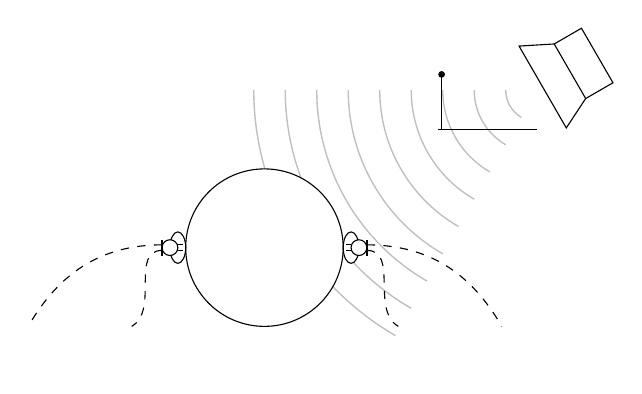
\begin{tikzpicture}
        \def\rad{4};
        \def\expand{1.02};
        \def\soundwavesegmentlength{0.4cm};
        \def\yscale{0.8};

        \begin{scope}[rotate around={30:(0,0)}]
            \pic[transform shape, scale=0.2] (right_speaker) at (\rad*\expand,0) {speaker};
        \end{scope}
        
        \draw[lightgray, decorate, decoration={expanding waves, angle=30, segment length=\soundwavesegmentlength}, line width=0.5pt] (30:\rad) -- (0,0);

        % Music producer
        \pic (producer) at (0,0) {head};

        % delta function
        \begin{scope}[xshift=2.2cm, yshift=1.5cm, draw=black]
            \draw[black] (0,0)--(1.26,0);
            \draw[black] (0.05,0)--(0.05,0.7);
            \filldraw[black] (0.05,0.7) circle (1pt);
        \end{scope}
        
        \begin{scope}[xshift=-3cm, yshift=-1cm, draw=black, xscale=0.02, yscale=\yscale]
            \node[minimum width=1.3cm, minimum height=1cm, anchor=west] (left_brir_box) {};
            \draw plot file {generated/brir_L.dat};
        \end{scope}
        \begin{scope}[xshift=1.7cm, yshift=-1cm, draw=black, xscale=0.02, yscale=\yscale]
            \node[minimum width=1.3cm, minimum height=1cm, anchor=west] (right_brir_box) {};
            \draw plot file {generated/brir_R.dat};
        \end{scope}

        \pic[transform shape, scale=0.1, rotate=90, local bounding box=left_mic] (left_mic) at (-1.2,0) {mic};
        \pic[transform shape, scale=0.1, rotate=-90, local bounding box=right_mic] (right_mic) at (1.2,0) {mic};

        \draw[dashed] ([yshift=1pt]left_mic.west) to[out=180, in=60, looseness=1] (left_brir_box.west);
        \draw[dashed] ([yshift=-1pt]left_mic.west) to[out=180, in=30, looseness=1] (left_brir_box.east);
        \draw[dashed] ([yshift=1pt]right_mic.east) to[out=0, in=120, looseness=1] (right_brir_box.east);
        \draw[dashed] ([yshift=-1pt]right_mic.east) to[out=0, in=150, looseness=1] (right_brir_box.west);
        
    \end{tikzpicture}

    \caption{Illustration of a binaural \gls{hrir} being recorded. An impulse is played back through the loudspeaker and recorded at microphones placed in each ear. The head acts a filter, altering the left and right microphone signals differently.}
    \label{fig:phantom_binaural}

\end{figure}


In traditional recording studio setups, the recording engineer or producer will use one or more microphones to capture an original sound source. These singular sound sources are commonly called \q{stems}. During the production process, the stems may be panned to create a sense of space in the final mix. In the case that the stem was recorded using two microphones, the stem would be called a \q{stereo stem}, and the term \q{panning} is usually replaced by \q{balance}, and only amplitude panning (as opposed to time or binaural panning) would be applied.

Amplitude panning is the most common panning technique in traditional music production \cite{shelvockHearingYourAudience2020}. It is associated with so-called \q{panning laws}, which govern how the amplitude is changed in each channel according the desired pan position \cite{izhakiPanning2023}. One example is the \q{energy-preserving pan law} (sometimes called the \mbox{\q{-3dB pan law}}) in which the squared sum of the channel gains always equals 1. The gains of the left and right channel are calculated by $g_L=\cos(\frac{\pi}{2}a)$ and $g_R=\sin(\frac{\pi}{2}a)$ respectively where $a$ is the panning position in the range $[0,1]$. \Cref{fig:equal_power_panning} shows how the channel gains relate to the panning position. The total perceived loudness will be equal at all panning positions.

\begin{figure}[hbt]
    \centering
    \includegraphics[scale=0.85]{equal_power_panning.pdf}\fxwarning[noinline]{Make it so that this diagram is full size but the final sentence still fits on the page.}
    \caption{Channel gains for equal power panning. When both channel gains are $\frac{1}{\sqrt{2}}$, the sound will be centre-panned. The perceived loudness is constant.}
    \label{fig:equal_power_panning}
\end{figure}

Panning techniques are applied to single stems only. A typical recording session will contain multiple stems, each with its own panning.

\subsection{Stereo image}
\label{sec:stereo_image}
The term \q{stereo image} is used to describe the overall distribution of sound across the horizontal plane after panning and any other production techniques have been applied on all stems. One may also use terms like \q{stereo field}, \q{soundstage}, or \q{panorama}, which all refer to the same thing. They are usually described in qualitative terms such as \q{big}, \q{wide}, and \q{ambient} rather than quantitative measures \cite{owsinskiMixingEngineersHandbook2006}. When mixing a musical recording, a producer will pan individual stems to their desired position within the stereo image. Those stems which are recorded in stereo have their own stereo image, which can also be controlled by the producer. The combination of all stems into a final stereo mix constitutes the overall stereo image. 

\Cref{fig:stereo_image} shows a simple example stereo image, as perceived by the producer. It contains two mono stems -- vocals and violin, and one stereo stem -- piano. There are some common tropes seen throughout many productions, some of which are shown in the diagram. Firstly, vocals are recorded in mono and panned to the centre. Secondly, since the piano is panned slightly left, the violin is panned roughly the same amount to the right in order to achieve a balanced mix. Thirdly, all stems are placed in the stereo image in a way that emulates a natural performance on a stage, and to avoid the instruments masking each other. Note that while these practices are commonplace, they are purely an artistic choice on behalf of the producer \cite{owsinskiMixingEngineersHandbook2006}; Recordings breaking the trend are not difficult to find.


\begin{figure}[htb]
    \centering

    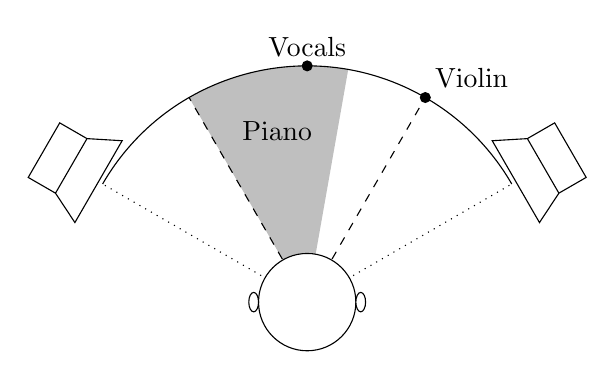
\begin{tikzpicture}
        \def\rad{3};
        \def\expand{1.02};

        \begin{scope}[rotate around={150:(0,0)}]
            \pic[transform shape, scale=0.2] (left_speaker) at (\rad*\expand,0) {speaker};
        \end{scope}

        \begin{scope}[rotate around={30:(0,0)}]
            \pic[transform shape, scale=0.2] (right_speaker) at (\rad*\expand,0) {speaker};
        \end{scope}

        % Piano
        \path[fill,lightgray] (0,0) -- (120:\rad)  arc (120:80:\rad) -- (0,0);
        \node at (100:2.2) {Piano};

        % Vocals
        \fill (0,0) (90:\rad) circle (2pt) node[above] {Vocals};

        % Violin
        \fill (0,0) (60:\rad) circle (2pt) node[above right] {Violin};

        % Stereo image
        \path[draw, dashed] (0,0) -- (120:\rad);
        \path[draw, dashed] (0,0) -- (60:\rad);
        \path[draw, dotted] (0,0) -- (150:\rad);
        \path[draw, dotted] (0,0) -- (30:\rad);

        % Draw full stereo image arc
        \draw (150:\rad) arc (150:30:\rad);

        % Music producer
        \pic[scale=0.618] (producer) at (0,0) {head};

    \end{tikzpicture}
    \caption{Example stereo image created by a music producer. Mono stems are shown as black dots and a stereo stem as a grey fill. Dashed lines represent the extent of the stereo image. Dotted lines represent the maximum boundaries of the possible stereo image.}
    \label{fig:stereo_image}
\end{figure}

\subsection{Production equipment and software}

To create a stereo image, a music producer will use the equipment available in a typical recording studio. Before the advent of digital recording, said equipment usually comprised a mixing console where each stem was assigned to one \q{track}. Each track had individual controls for (amongst others) level and panning that were directly linked to the internal electronics. The producers might also use the term \q{fader} for the level control and \q{pan-pot} for the panning control\footnote{The term \q{pan-pot} is a shortening of \q{panoramic potentiometer}.}. All tracks would be mixed by the console and the combined output fed to stereo speakers for playback. In a digital recording studio, the equipment is largely the same except that the mixing console will be connected to a computer that controls the session and stores the recorded audio. \Cref{fig:recording_studio} shows photographs of a small recording studio where the faders and pan-pots for each track are visible. The music producer will manipulate the physical controls for each track to create a stereo mix.

\begin{figure}[hbt]
    \centering
    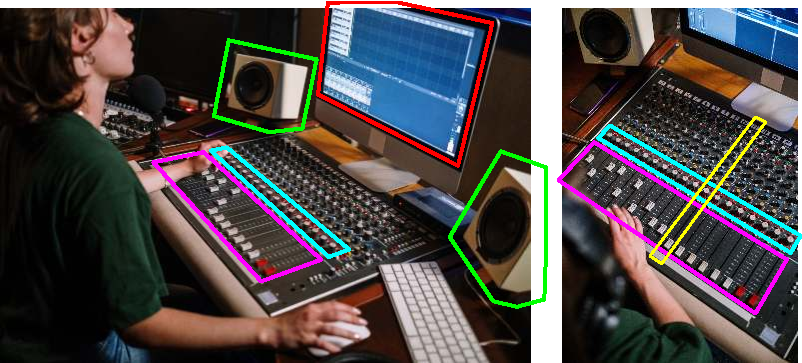
\includegraphics[width=\linewidth] {figures/studio_photos_small.pdf}
    \caption{Photographs of a small recording studio\textsuperscript{*}. The left photo shows all studio equipment, while the right photo shows a close-up of the mixing console. Faders are highlighted pink, pan-pots are highlighted blue, stereo speakers are highlighted green, and the computer running a \glsfmtfull{daw} is highlighted red. One track is highlighted yellow.}
    \label{fig:recording_studio}
    \begin{flushleft}{\scriptsize\textsuperscript{*}\href{https://www.pexels.com/photo/a-person-in-green-crew-neck-t-shirt-sitting-infront-of-computer-and-audio-mixer-5657660/}{Original} \href{https://www.pexels.com/photo/person-using-audio-mixer-5657676/}{images} by cottonbro studio are licensed under \href{https://www.pexels.com/license/}{Pexels}. Annotations have been added.}\end{flushleft}
\end{figure}

In modern recording scenarios a music producer typically uses a \gls{daw} - graphical software that allows them to record and edit audio. There are many \glspl{daw} available, but one such example (Reaper) is shown in \cref{fig:daw}. In particular, it shows a single recorded audio track which has its \q{Pan} control automated. In a more complete recording session, the \gls{daw} would contain many more tracks, each with their own pan control.

\begin{figure}[p!]
    \centering
    \begin{subfigure}[b]{\textwidth}
        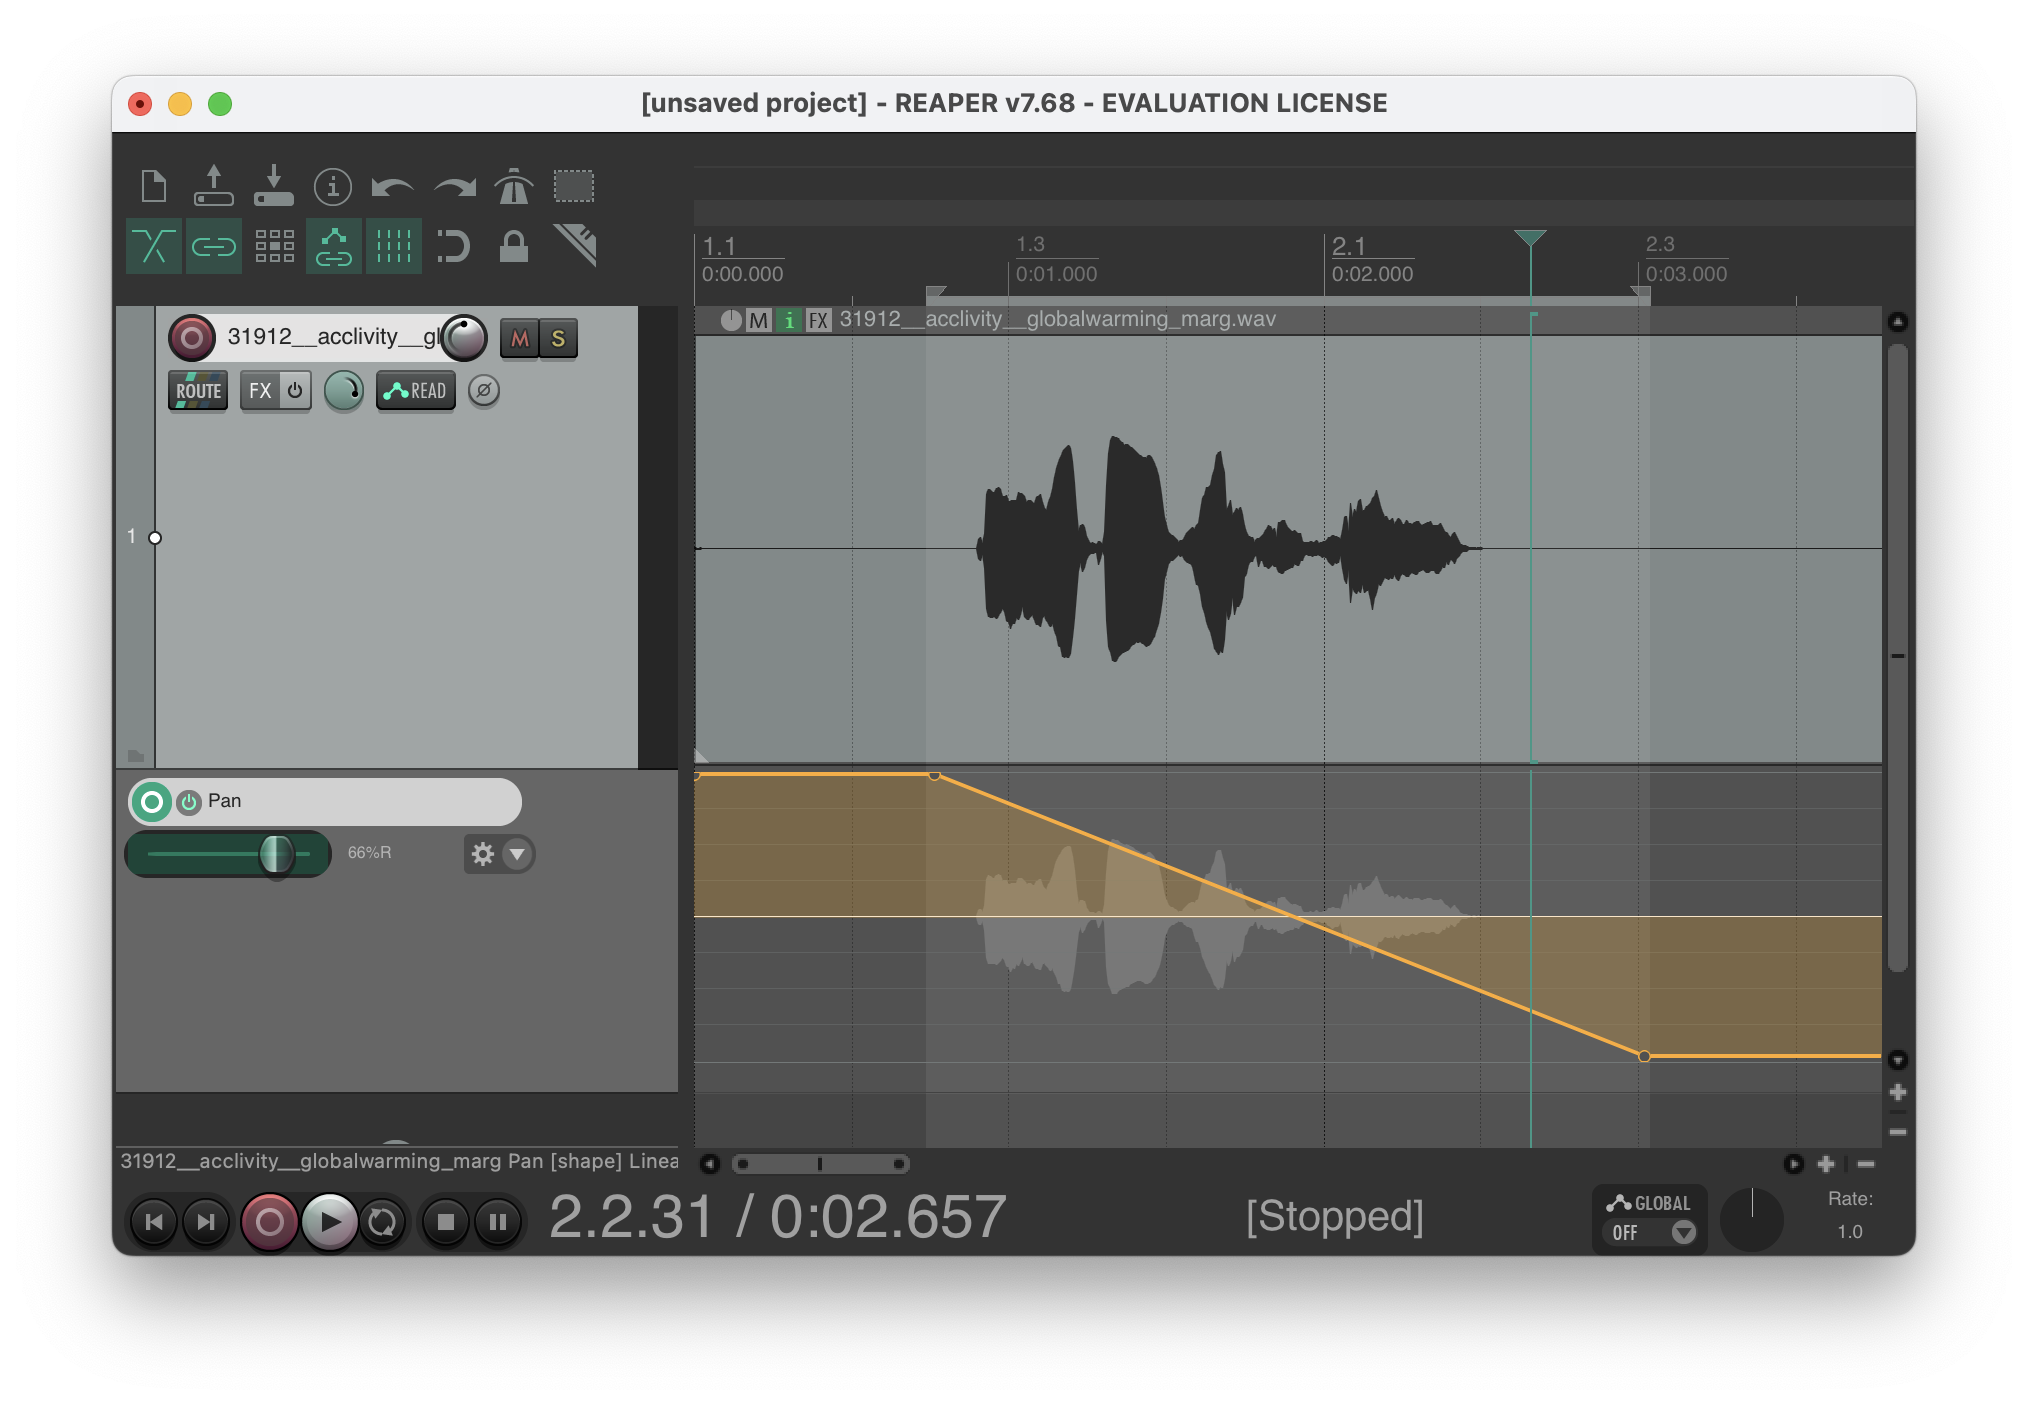
\includegraphics[width=\linewidth]{figures/daw.png}
        \caption{Recording project in the Reaper \gls{daw} \cite{REAPERAudioProduction}}
        \label{fig:daw}
    \end{subfigure}

    \bigskip
    
    \begin{subfigure}[b]{\textwidth}
        % \centering
        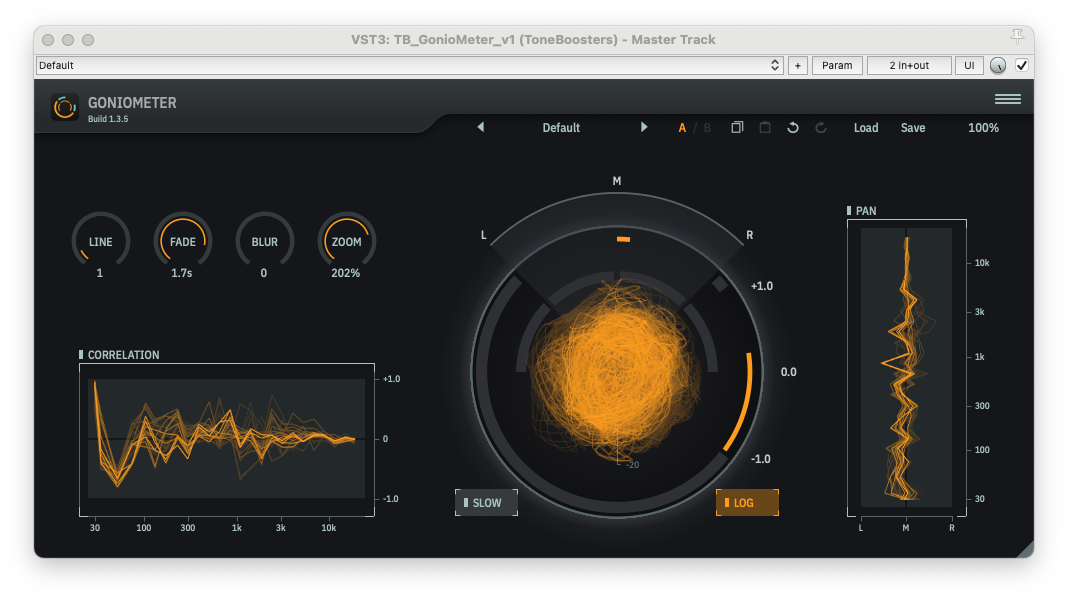
\includegraphics[width=\linewidth]{figures/goniometer_plugin.png}
        \caption{ToneBoosters Goniometer plugin \cite{ToneBoostersAudioPlugins}}
        \label{fig:goniometer}
    \end{subfigure}
    \caption{Screenshots of example music production tools}
\end{figure}

While there are some typical practices in the industry, it must again be emphasized that panning and creation of stereo field more generally is an artistic process \cite{izhakiPanning2023}. The producer pans each track individually by either physically turning the \mbox{pan-pots} or adjusting a digital panning control, and judges the stereo image purely by listening. Producers are typically known for their individual style and taste, and the ways in which they use panning in a large \gls{daw} session containing many tracks forms part of that style.

In some cases the producer consults monitoring equipment such as a level meter or goniometer to fine tune their mix \cite{ziemerAcousticFeaturesRecording2021,ziemerGoniometersArePowerful2023}. They also look for potential quality issues that can occur when the stereophonic recordings are mixed down into a monophonic signal for reproduction, which have been documented well before the advent of digital recording \cite{harveyCompatibilityProblemsTwochannel1962}. In more modern production, \gls{daw} plugins are generally used to visualize and assess the stereo qualities of the final mix \cite{bitzerSpatialDistributionMeter2007,ziemerGoniometersArePowerful2023}. \Cref{fig:goniometer} shows one example - the ToneBoosters Goniometer plugin \cite{ToneBoostersAudioPlugins}. It is designed to replicate an analogue goniometer, which, taking two voltage signals as input, displays them on a 2D axis such that a music producer might be able to discern the correlation between the signals.


\subsection{Audio representations}
Audio representations are standard paradigms that an audio recording can follow. If we consider an audio recording as a set of concurrent time signals, the representation defines how each signal in the set should be interpreted. They are usually grouped into \q{channel-based}, \q{scene-based}, and \q{object-based}. In channel-based audio, each signal represents the exact waveform that should be played back by a single loudspeaker. In scene-based and object-based audio, each signal represents one part of a larger scene, and rendering equipment is responsible for translating that scene to individual speakers \cite{sugimotoSpecificationAudioRepresentations2024}. While the focus of this thesis in on stereo audio, it is important to compare stereo to the wider audio landscape to understand why it is so heavily used for recorded music.

\subsubsection*{Monophonic}
Monophonic recordings contain a single channel to be played back on one speaker. They are only able to convey a small amount of spatial information; reverberation is the only way to infer a sense of space. Archival/historical recordings will be recorded in mono, as well as a majority of raw studio stems, speech, and telephony recordings.

\subsubsection*{Stereophonic}
Stereo recordings contain two channels: left and right. Compared to mono, stereo has the ability to convey the width and location of a sound 2D space. For music this sense of space is especially important since music signals tend to be highly dense and complex. Stereo mixing therefore allows music producers to add clarity and balance to their recordings. This marked increase in quality drove stereo's commercial adoption in the 1950s, and it has been the dominant format for recorded music since then \cite{lanierHIFITWOCHANNELCOMMOTION1957}.

\subsubsection*{Binaural}
Binaural can be considered a subset of stereo. Each channel conveys the precise sound wave as heard at the left and right ears. It is typically used when rendering spatial audio\footnote{The exact definition of \q{spatial audio} is somewhat contested in the literature but here I assume \citeauthor{cobosOverviewMachineLearning2022}'s definition: \textit{\q{audio that contains spatial information}} \cite{cobosOverviewMachineLearning2022}.} for playback on headphones, and in \gls{vr} or \gls{ar} scenarios.

\subsubsection*{Multichannel}
Multichannel is a continuation of stereo which adds speakers at more positions. While it could contain any number of channels, there are some standards that are referred to by their channel count and layout, e.g. 5.1 (5 listener-plane channels, 1 \gls{lfe} channel) or 22.2 (10 listener-plane, 2 \gls{lfe}, 9 overhead, 3 low) \cite{sugimotoSpecificationAudioRepresentations2024}. Compared to stereo, it has the ability to convey width, depth, and -- depending on the arrangement -- height, creating a higher sense of immersion. This ability sees it being used mainly for film and TV soundtracks where the emotional impact of single sound events can be critical. That said, the high setup cost and difficulty positioning extra speakers has historically discouraged its wider adoption \cite{bayleySurroundSoundDAW2012}.

\subsubsection*{Ambisonics}
Ambisonics is a scene-based audio representation where each channel is one directional component of a 3D physical sound field. Recordings are referred to by their \q{order}, which implies both the number of different directions and the number of channels. The number of required channels increases quadratically with the order according to the formula $C=(O + 1)^2$ where $C$ is the number of channels and $O$ is the order. Ambisonics typically excels at representing diffuse sounds, but struggle to represent point sources unless the order is very high. Thus, ambisonic recordings are only used for very specific types of music, such as orchestral performances in large concert halls where accurate recreation of the ambience is more important than individual instruments. Even in those cases, an ambisonic recording will generally be rendered to binaural for mass distribution \cite{churnsideAmbisonicsPeriphony2010}.

\subsubsection*{Object-based audio}
In object-based audio, the entire audio scene is composed of individual audio objects accompanied by metadata specifying their location and movement. Rendering equipment is then responsible for translating those objects to speaker channels for playback. It is a relatively new format and while its main use is for cinematic sound, the music industry has recently begun to adopt it. In contrast to ambisonic recordings, object-based audio is distributed in its original form, allowing the same set of signals to be rendered in multiple ways.
\\\\
Overall, stereo recordings are able to deliver high enough quality for the majority of music listeners. The newer formats, while gathering interest in pockets of the music community, have yet to receive wide-spread adoption from consumers. The result is that the mainstream distribution of music still happens in stereo.

\subsection{Lossless and lossy encoding}
Regardless of which audio representation is chosen, the resulting recording will most likely be encoded to a compressed format for distribution. There are two types of compression: \q{lossless} and \q{lossy}. A lossless format, when decoded, will produce bit-for-bit recreation of the input signal. Lossy formats on the other hand will not produce the exact same signal, but will discard information that they consider irrelevant according to a psychoacoustic model. There are many lossy formats each suitable for different types of audio, but for the purposes of this thesis it is just pertinent that spatial information can be lost during lossy encoding.

% \clearpage

\section{Analysis of digital recordings}

The output of a recording session is usually only the stereo mix. Stems and \gls{daw} sessions are generally kept private, with precious few being available under licensing terms that are conducive to academic research \cite{bittnerMedleyDBMultitrackDataset2014}. Thus, we assume that all analysis can only be performed on the final stereo mixes that are distributed for playback. The most common distribution format is a digital audio file, and there are some fundamental analysis techniques that can be applied to a digital audio signal.

\subsection{Digital audio signals}
When a sound wave interacts with a microphone, it generates an electrical signal in continuous time. To convert that analogue signal into a digital one, it is sampled at regular intervals. The sampling frequency ($f_s$) is related to the sampling interval ($T_s$) by the relationship $T_s = \frac{1}{f_s}$.

Shannon's sampling theorem states that a signal can be perfectly recreated when sampled at twice the highest frequency contained in the signal. Conversely, the highest frequency that can be represented by sampling a signal at a given $f_s$ is half of that frequency. This limit is called the \q{Nyquist frequency} and is calculated by $f_N = \frac{f_s}{2}$ \cite{yaoNyquistFrequency1983}. This is illustrated by \Cref{fig:nyquist}, which shows the sampling of three waveforms. The lower plot shows a signal at the Nyquist frequency ($f_N$), which can be perfectly reconstructed from the digital samples. The upper two waveforms have frequencies equidistant but in opposite directions from the Nyquist frequency ($f_N \pm f_{\delta}$). The digital samples shown in circles could represent either of the two waveforms. In practice, when the analogue waveform is reconstructed, the lower frequency will always take precedence. 

\begin{figure}[t!]
    \centering
    \includegraphics{nyquist.pdf}
    \caption{Illustration of the Nyquist Frequency in digital audio signals. Dotted vertical lines represent sampling points with a separation of $T_s$, and monotonically increasing index $n$. The upper plot shows a cosine wave at exactly $f_N$. The lower plot shows two cosine waves with frequencies equidistant above and below the Nyquist frequency ($f_N$). Sampled values are shown as circle marks on the plots. The two upper signals can both be represented by same digital samples.}
    \label{fig:nyquist}
\end{figure}

A typical $f_s$ for music is \qty{44.1}{\kHz}, with a resulting $f_N$ of \qty{22.05}{\kHz}. The prevalence of this particular number stems from the first widespread distribution mechanism for digitally encoded music - the \gls{cd}\footnote{\qty{44.1}{\kHz} was chosen by a consortium of \gls{cd} manufacturing companies as a trade-off between technical requirements and the limits of human perception \cite{baertDigitalAudioCompact2013}.}. While higher frequencies may be used in the recording and production process, an exceedingly large proportion of recorded music has been distributed at \qty{44.1}{\kHz}, even after \glspl{cd} were displaced by other distribution methods.

\subsection{Time-Frequency representation of audio}

In order to perform many types of audio analysis, the audio signal can be converted from the time domain into the \gls{tf} domain. In perceptual acoustics research there are several common forms of \gls{tf} representation, each with its own nuances. This section provides those details, and a side-by-side comparison is shown at the end of the section in \cref{fig:spect_comp}.

\subsubsection{\gls{stft} spectrogram}

The \gls{stft} spectrogram is one of the most popular \gls{tf} representions across all audio processing work due to its computational efficiency. The fundamental principle is that a time-domain signal is split into short (1 to 100ms) overlapping chunks, and the \gls{fft} is performed on each chunk, thereby converting that chunk into the frequency domain.  By arranging subsequent frames along a time axis it is possible to represent the original signal as a 2D image known as a spectrogram. When the time-domain signal is entirely real, (which is the case for monophonic audio signals), the result of the \gls{fft} will be a complex signal which is symmetrical around the Nyquist frequency and the upper half is therefore dropped. Furthermore, the complex spectrum is usually represented in magnitude/phase form to better match the human auditory response.

A fundamental property of the \gls{fft} is that it assumes that the signal repeats outside the time frame that is being analysed. Since this is generally not the case for audio signals, it is standard practice to apply a time-domain windowing function to each frame so that large transients do not occur at the boundaries. Several standard windowing functions exist, each with their own nuances, but for most audio applications the \q{Hann} window can be used \cite{LibrosastftLibrosa0110}. 

The nature of the spectrogram is affected by two parameters: the frame size and hop size. \q{Frame size} refers to the number of samples in each analysis frame. To obtain maximal computational efficiency this must be a power of 2. \q{Hop size} refers to the number of samples between the start of subsequent frames and is sometimes expressed as a percentage of the frame size. The frame size dictates the resolution of the spectrogram's frequency axis since the frequency bins will be spaced evenly between \SI{0}{\hertz} and the Nyquist frequency. Importantly, a longer frame size will result in lower time accuracy within each frame; sharp transients in the time domain will appear as wideband energy in the frequency domain, but information about exactly where the transient occurred within the frame is lost. To counteract this inaccuracy, a smaller hop size can be used so that transients might be detected as sharp changes between \gls{stft} frames. One major drawback of the \gls{stft} spectrogram is that the linearly-spaced frequency bins do not align well with the human perception of frequency, which is logarithmic. The \gls{stft} therefore contains redundant information in higher frequencies. Several common alternatives exist to account for this.

\begin{figure}[htb]
    \centering
    \includegraphics{stft_spect.pdf}
    \caption{\gls{stft} spectrogram of a speech recording.}
    \label{fig:stft_spect}
\end{figure}

\subsubsection{Mel spectrogram}

The \q{Mel scale} is a quasi-logarithmic frequency scale derived from perceptual experiments. Several definitions exist in the literature \cite{umeshFittingMelScale1999}, but popular implementations like that of librosa \cite{mcfeeLibrosaAudioMusic2015} and \gls{amt} \cite{majdakAMT1xToolbox2022} tend to underpin most audio experimentation.

A \q{Mel filter bank} is a set of band-pass filters that are spaced equally on the Mel scale. Practically, they are implemented as sets of weights that are applied to an \gls{stft} spectrum with the relationship $M_n = \sum_{k=0}^{N} S_k W_{k,n}$ where $M_n$ is the $n$th Mel coefficient, $S_k$ is the $k$th \gls{stft} bin, $N$ is the number of \gls{stft} bins, and $W_{k,n}$ is the $k$th weight of the $n$th Mel filter. An example Mel filter bank with 8 filters is shown in \cref{fig:mel_filters}. While 8 filters are shown for demonstration purposes, audio analysis typically requires over 100. When this filter bank is applied to each time step of an \gls{stft} spectrogram, the result is a \q{Mel spectrogram}, an example of which can be seen in \cref{fig:mel_spect}. Observe that the higher frequencies have been condensed into fewer frequency bins compared to the \gls{stft} spectrogram.


\begin{figure}[b!]
    \centering

    \begin{subfigure}[h]{\textwidth}
        \centering
        \includegraphics{mel_filterbank.pdf}
        \caption{Example Mel filter bank containing 8 filters, shown with linear (left) and logarithmic (right) frequency scales. The bandwidth of each filter is roughly equal in logarithmic space, and the amplitudes are scaled so that the sum of the weights in each band is equal. Filter weights equal to zero are removed for clarity. 
        % The filters are calculated using librosa \cite{LibrosafiltersmelLibrosa0110} using a sample rate of \SI{44100}{\hertz} and an \gls{fft} size of 4096 samples.
        }
        \label{fig:mel_filters}
    \end{subfigure}

    \bigskip

    \begin{subfigure}[h]{\textwidth}
        \centering
        \includegraphics{mel_spect.pdf}
        \caption{Mel spectrogram of a speech recording, using 32 bands.}
        \label{fig:mel_spect}
    \end{subfigure}
\end{figure}

\subsubsection{Cochleagram}

As an alternative to the two spectrogram representations, a cochleagram aims to make a \gls{tf} representation that models the acoustic response of the human cochlea more closely. To that end, all processing is performed in the time domain and is sometimes referred to as a \q{peripheral ear model}. Several examples appear in the literature \cite{boddenBinauralModelingAuditory1995,choiObjectiveMeasurementPerceived2008,delgadoDesignChoicesBinaural2023}. In the classical method \cite{boddenBinauralModelingAuditory1995} the original signal is first processed by a bank of gammatone filters with their centre frequencies placed according to a perceptual scale (such as the \gls{erb} scale \cite{smithiiiEquivalentRectangularBandwidth2020}), as shown in \cref{fig:gammatone_filters}. As with Mel filters, several definitions of gammatone filters exist in the literature, but the popular implementations (e.g. scipy \cite{virtanenSciPy10Fundamental2020} and \gls{amt} \cite{majdakAMT1xToolbox2022}) preside. \Cref{fig:cochleagram} shows a cochleagram of the example speech recording.

\Cref{fig:cochleagram_steps} shows the intermediate steps to generate a cochleagram. Each sub-band signal is processed by a half-wave rectifier, square root, and low-pass filter to mimic the excitation patterns of the cilia and basilar membrane. The result is a signal representing the envelope of each sub-band. Those envelopes are then segmented into overlapping time chunks. The amplitude of each chunk is then calculated as the mean of all its values, forming one pixel in the cochleagram.

\begin{figure}[hbt]
    \centering
    \includegraphics{cochleagram.pdf}
    \caption{Cochleagram of a speech recording, using 32 bands.}
    \label{fig:cochleagram}
\end{figure}

\begin{figure}[p!]
    \centering
    \begin{subfigure}[b]{0.8\textwidth}
        \centering
        \includegraphics{gammatone_filterbank.pdf}
        \caption{Example gammatone filter bank with individual filters spaced equally on the \gls{erb} scale. The filters are \glsentryfull{iir} and are applied to an audio signal in the time domain.}
        \label{fig:gammatone_filters}
    \end{subfigure}

    \begin{subfigure}[b]{\textwidth}
        \includegraphics{cochleagram_steps.pdf}
        \caption{Steps of an example decomposition from time-domain audio to a cochleagram. The audio being filtered is a frequency sweep from 100 to 20000 Hz. First it is processed by a gammatone filter bank, generating 8 sub-band signals which are spaced equally on the \gls{erb} scale. Each sub-band has its envelope extracted. The envelope is then split into overlapping time chunks, which are averaged to form the cochleagram.}
        \label{fig:cochleagram_steps}
    \end{subfigure}
    \caption{Using a gammatone filter bank to make a cochleagram.}
\end{figure}


\begin{figure}[p!]
    \centering
    \includegraphics{spect_comp.pdf}
    \caption{An example audio signal displayed as \gls{stft} spectrogram (above), Mel spectrogram (mid), and cochleagram (below). The spectrogram frequency bands are spaced linearly between 0Hz and the Nyquist frequency, which is not coherent with human perception. The Mel spectrogram is created from the original spectrogram based on linear combinations of its frequency bands and retains more detail in lower frequencies than higher frequencies. The Cochleagram is created directly from time domain audio by mimicking the physical response of the human ear.}
    \label{fig:spect_comp}
\end{figure}

\pagebreak

\subsection{Machine learning}
Any data-driven audio research, particularly that using vast datasets, will naturally involve the use of \gls{ml}. Broadly speaking, \gls{ml} techniques can be classified as either supervised or unsupervised. When training a supervised  \gls{ml} model, the training dataset needs to include ground-truth labels such that the network can objectively discern via a loss function whether the predictions it is making are correct. Unsupervised \gls{ml} on the other hand does not require any labels. Instead, it seeks to form a representation of the underlying dataset via techniques such as clustering or dimensionality reduction, thereby learning the structures and patterns of the data while retaining as much key information as possible.

Striking a middle ground between the two is \q{self-supervised} learning, which addresses the issue of creating objective ground-truths from unlabelled data. Instead of relying on external labels, self-supervised learning generates pseudo-labels from the dataset itself, and then uses those as the input to a \q{pretext task}, which is tackled in much the same way as a supervised task.

As an example we can consider the current largest dataset of recorded music: \gls{fma} \cite{defferrardFMADatasetMusic2017}. The dataset contains the stereo audio of approximately \num{100000} tracks, along with metadata such as genre tags. An unsupervised task might involve learning a high-order representation of the raw spatial cues present in the stereo signals. A supervised task might involve predicting genre using the audio signal as input. A self-supervised task might involve masking off a short period of audio and filling it back in using the surrounding audio as context. 

In relation to the \hyperref[sec:research_questions]{overarching \gls{rq}} in \cref{sec:research_questions}, we assume that a music producer's \gls{daw} session is the only source of objective ground-truth data regarding stereo field. Furthermore, we assume that \gls{daw} sessions are not publicly available, as was found in \cite{colonelReverseEngineeringRecording2021,rodriguezSpectralDynamicConstellations2024}; The only public-facing output of a recording session is the mixdown. It follows that either unsupervised or self-supervised learning is necessary to draw any conclusions to the \glspl{rq}.




\chapter{Related works}
\label{sec:related_works}

In this chapter I break down the details of existing algorithms for stereo field analysis, as well as demonstrating those techniques on example audio recordings. To provide additional context, I also present several high-level initiatives within the audio industry, showing how stereo field analysis has been used up until the present day. Throughout the chapter I use 3 recordings as examples. They all come from the \gls{fma} dataset \cite{defferrardFMADatasetMusic2017}, and each one presents a different use of stereo image. In the text they are referred to simply as track \q{A}, \q{B}, and \q{C}. Full details for all tracks can be found in appendix \ref{app:demo_tracks}. Note that in order to discuss and demonstrate the algorithms in this chapter, I implemented them from scratch in a monolithic software library. By breaking each algorithm down into its constituent parts it was possible to draw links between them, since they often share underlying \gls{dsp} techniques.

\section{A brief history of stereo field in industry}
\label{sec:history}
Research into the stereo field of recorded music specifically (as opposed to generic spatial properties of audio signals) has its roots in the early 2000s. At the time, stereo recording was a well-established norm and audio distribution was handled by the early lossy encoding formats such as \gls{mp3} and \gls{aac} \cite{iso-11172-3:mpeg_audio,ISOIEC13818-7:2006-AAC}. Analysis and description of stereo field was used to increase the coding efficiency of these codecs, for example by e.g. \gls{ps} coding \cite{fallerParametricCodingSpatial2004,breebaartHighqualityParametricSpatial2004,breebaartParametricCodingStereo2005}. In parallel, new audio encoding schemes such as \gls{bcc} (later ratified as \q{\glsxtrshort{mpeg} Surround} \cite{iso/iec23003-1InformationTechnologyMPEG2007}) were developed based on the work of \citeauthorandnumber{baumgarteEstimationAuditorySpatial2002}. 

The standardization of multichannel audio presented an opportunity: new reproduction equipment needed to remain compatible with the existing back-catalogue of stereo recordings, and vendors could compete on sound quality. There was therefore a need algorithms that upmixed stereo audio to multichannel. Analysis of the stereo field, source separation, and primary/ambient extraction were seen as effective ways to achieve this \cite{goodwinPrimaryAmbientSignalDecomposition2007}. In fact, such research is still ongoing today \cite{shiFastNonuniformSearching2022}.

In the prevailing years, object-based audio has been developed and standardized as e.g. Dolby Atmos \cite{DolbyAtmosNextGenerationAudioforCinema} and MPEG-H \cite{mpeg-h}, and the same early research into stereo field analysis is still relevant to these new formats for all the same reasons. Nowadays, it is commonplace to use \gls{ml}/\gls{dl} to perform the same tasks, although the results only outperform the \gls{dsp}-based predecessors in specific cases \cite{cobosOverviewMachineLearning2022}.

With access to these efficient distribution formats, large digital music collections emerged and brought new problems to solve: collectors needed ways organize and categorize their music. Stereo field analysis was just one of the mechanisms used to facilitate this, paving the way for research into e.g. \gls{agr}, \gls{mir}, and music recommendation \cite{guausAudioContentProcessing2009,harmaClassificationTimefrequencyRegions2010,defferrardFMADatasetMusic2017}.

\section{Spatial cues for stereo image}
\label{sec:spatial_cues}

A \q{spatial cue} is a low-level analysis of spatial information in a short (roughly 1-100ms) audio snippet. While those mentioned in \cref{sec:directional_hearing} aim to describe binaural sound as perceived by humans, there are several examples of spatial cues tailored specifically to the analysis of recorded music.

The \q{panning index} and \enquote{ambience index} specified by \citeauthor{avendanoFrequencyDomainTechniques2002} \cite{avendanoFrequencyDomainTechniques2002} are loosely analogous to \gls{ild} and \gls{iacc} in the acoustics domain. To estimate the \q{panning index}, a signal model is assumed whereby a musical source is panned within the mix using the \enquote{energy preserving pan law}, in which each channel is scaled such that the sum of the squared amplitudes equals 1 (see \cref{sec:panning}). While this panning technique does not affect the phase of either channel, existing phase differences between channels are measured using the \q{ambience index}, which is defined such that it is low when the stereo channels are correlated (indicating a direct sound source), and high when channels are uncorrelated (indicating an ambient or reverberant sound source). An example of the panning and ambience indices for a musical recording can be seen in \cref{fig:pi_ai}.

\begin{figure}[!p]
    \centering
    \includegraphics{pi_ai.pdf}
    \caption{Demonstration of \pani{} and \ambi{} on Track C. Several panned sources are visible as red or blue bands in the \pani{}, and at roughly 20s most sources fade out leaving a single one on the right. The \ambi~plot shows that the track starts off with no single dominant direct sound source. At 20s when most sources fade out, the \ambi~drops to 0 across the lower half of the spectrum, indicating that the remaining source is direct. In the upper half of the spectrum, the source remains slightly ambient. }
    \label{fig:pi_ai}
\end{figure}

\citeauthor{prestiBivariateMixtureSpace2023} provides a re-contextualization of the panning and ambience indices in his work on \glspl{bms} \cite{prestiVisualizationManipulationStereophonic2014,prestiBivariateMixtureSpace2023}. He demonstrates that it can be used to analyse the panning position of individual \gls{tf} bins, plus the clarity (or trustworthiness) of that measurement. Thus, it is useful for tasks such as primary/ambient decomposition, stereo field manipulation, and visualization.

\citeauthor{barrySoundSourceSeparation2004} present another seminal technique in their paper defining the \gls{adress} algorithm \cite{barrySoundSourceSeparation2004}. The fundamental principle is to estimate the panning position of frequency bins in a stereo spectrogram by scaling one channel, inverting it, and mixing the channels back to mono. The resulting phase cancellation will determine the scaling factor that was applied to the original audio source during amplitude panning, and hence will show where the source was panned in the stereo field. To demonstrate, \cref{fig:adress} shows an example \gls{fa} plane for a combination of panned sine waves, where nulls in the plane show can be observed at the azimuths position that the sinusoids are panned to. To show a realistic use case, \cref{fig:faas} shows an \gls{fa} analysis signal for a music recording. While this was technique was originally intended to be used for audio source separation, it has been repurposed many times since.

Importantly, all the previously mentioned analyses are performed in the \gls{tf} domain and result in one value per \gls{tf} bin. Their use cases typically involve reconstruction or editing of the original audio source as opposed to \textit{description} of it since they inherently entangle semantic content with spatial information. They have, however, become the basis of other algorithms that are designed specifically for description.

\begin{figure}[hbt]
    \centering

    \begin{subfigure}[b]{\columnwidth}
        \includegraphics{adress.pdf}
        \caption{\gls{fa} plane for a signal comprising 8 sinusoids at differing frequencies. Half are panned left and half are panned right. Red dashed lines show the panning positions detected by looking for nulls in the \gls{fa} plane. This \gls{fa} plane is formed from a single frame of an \gls{stft} spectrogram.}
        \label{fig:adress}
    \end{subfigure}

    \vspace{2em}

    \begin{subfigure}[b]{\columnwidth}
        \centering
        \begin{tikzpicture}[
            frame/.style={
                yslant=0.5,
                minimum width=0.618in,
                minimum height=0.618in,
                draw=black,
                inner sep=0pt,
                outer sep=6pt,
            },
        ]
            \foreach \x in {0, 1, ..., 7} {
                \node[frame] (a-\x) at (1.25*\x, 0) {
                    \includegraphics[
                        width=0.618in,
                        height=0.618in
                    ]{fa_0000\x.png}
                };
            }
            
            \draw[arrow] (a-0.south west) -- (a-7.south west -| a-7.south east) node[pos=0, left] {\small Time};
        \end{tikzpicture}
        \caption{\gls{fa} analysis signal constructed from consecutive \gls{fa} planes of track C.}
        \label{fig:faas}
    \end{subfigure}

    \caption{\glsxtrfull{fa} planes and analysis signal.}
    
\end{figure}

\pagebreak

\section{Stereo image description}
\label{sec:stereo_image_description}

Stereo image description refers to the generation of a numerical vector that represents the stereo image in an arbitrary feature space. Recordings with similar stereo image should be close within the space, although the distance metric is application-specific. A typical technique is to construct the vector from statistical summaries of low-level spatial cues. In the acoustics domain where stereo image description is typically used for analysis of concert halls and music reproduction systems, the previously mentioned spatial cues (\gls{ild}, \gls{itd}, and \gls{iacc}) typically form the basis of the analysis. However, as stated by \citeauthor{sarroffComputationalModelPerceived2011}, the task of describing recorded music is inherently different since said recordings may exhibit spatial aspects that cannot occur in physical acoustic space \cite{sarroffComputationalModelPerceived2011}. Throughout this section, these descriptions are referred to as \glsxtrfullpl{sip}, and examples of each one are given on the three example tracks.


\subsection{\glsentryshort{dsp}-based \glsentryshortpl{sip}}

\citeauthor{tzanetakisStereoPanningFeatures2007} provide the earliest example of a technique specifically designed to interpret the use of panning in recorded music: \gls{spf} \cite{tzanetakisStereoPanningFeatures2007}. It targets amplitude panning only, using \citeauthor{avendanoFrequencyDomainTechniques2002}'s \pani{} as the basis. Additionally, it separates the frequency spectrum into 3 sub-bands -- lows, mids, and highs -- following the common practice of music producers. While not specifically stated by \citeauthor{tzanetakisStereoPanningFeatures2007}, I interpret the vector to represent the amount and variance of \q{fast panning} and \q{slow panning} in each frequency band. \citeauthor{tzanetakisStereoPanningInformation2010} later expanded the features by adding an estimation of the number of individual sources in the recording \cite{tzanetakisStereoPanningInformation2010}. The resulting \gls{sip} can be used to compare the recording and production styles of different music tracks, as shown in \cref{fig:spf}.

\begin{figure}[p!]
    \centering
    \includegraphics{spf.pdf}
    \caption{
        \glsentrylong{spf} for three tracks from the \gls{fma} dataset \cite{defferrardFMADatasetMusic2017}. All tracks clearly show different panning and production styles. 
    }
    \label{fig:spf}
\end{figure}

While \gls{spf} shows production style at a high level, other descriptors contain more detail. \citeauthorandnumber{gomezMusicSimilaritySystems2008} and \citeauthorandnumber{sarroffMeasurementsSpaciousnessStereophonic2008} both present separate methods to form a \gls{ph}, which displays the likelihood of a sound source being panned to a specific azimuth. \Cref{fig:panning_histograms} shows examples of both methods for the same three example tracks. As \citeauthor{sarroffMeasurementsSpaciousnessStereophonic2008} state, the \q{azimuth} value should not be interpreted as a true angular position relative to the listener, but rather as a loose placement of a sound source within the stereo field. Note that compared to \gls{spf}, \gls{ph} visualizes the exact location of sound energy in the stereo field rather than just the \q{amount of panning}. On the other hand, \gls{ph} looses information about the \textit{dynamics} of the panning, which \gls{spf} does not. \citeauthor{sarroffMeasurementsSpaciousnessStereophonic2008} subsequently use the \gls{ph} to calculate an estimate of stereo width \cite{sarroffMeasurementsSpaciousnessStereophonic2008}, which is an important perceptual measure (see \cref{sec:prediction_of_perceptual_scalars}).

\begin{figure}[p!]
    \centering
    \includegraphics{panning_histograms.pdf}
    \caption{
        \glsentrylongpl{ph} for three tracks from the \gls{fma} dataset \cite{defferrardFMADatasetMusic2017}. All tracks clearly show different shapes of stereo field. The two different algorithms (\citeauthorandnumber{gomezMusicSimilaritySystems2008} and \citeauthorandnumber{sarroffMeasurementsSpaciousnessStereophonic2008}) produce slightly different fine detail, but they agree on the general azimuthal distribution.
    }
    \label{fig:panning_histograms}
\end{figure}

\FloatBarrier

\citeauthor{gomezMusicSimilaritySystems2008} present a continuation of their \gls{ph} algorithm. They note that the histogram itself can be quite large, and that standard distance metrics may not correlate with perceptual differences. To avoid this, they propose converting the \gls{ph} to a vector of \q{\gls{pc}} in a non-perceptual domain and truncating it. \Cref{eq:cepst_ph} shows this conversion where $\vec{C}$ is the vector of coefficients, $\mathcal{F}^{-1}$ is the inverse \gls{fft}, $L$ is the truncation length, and $\vec{H}\vec{H}^{\leftarrow}$ is a concatenation of the panning histogram and its reverse. 

\begin{equation}
    \vec{C} = \left\{\mathcal{F}^{-1} \left\{ \log (\vec{H}\vec{H}^{\leftarrow})\right\} \right\}_{1:L}
    \label{eq:cepst_ph}
\end{equation}

The efficacy of this technique remains under-tested, and my work in paper \ref{paper:dafx} showed that \gls{pc} were unable to accurately represent \glspl{ph} with sharp peaks. It should also be noted that, as revealed by paper \ref{paper:slr}, the term \q{\glsxtrlong{pc}} is used frequently in the literature to mean other things \cite{liUnsupervisedAdaptiveFiltering2005,chunFrequencyDependentAmplitudePanning2016,miethObjectiveEvaluationTechniques2017,cabanas-moleroMusicDemixingMachine2023}. 


\citeauthor{tardieuProductionEffectAudio2011} present another assessment of amplitude panning named \gls{asf} \cite{tardieuProductionEffectAudio2011}. Differing from the previously mentioned techniques, \citeauthor{tardieuProductionEffectAudio2011}'s method focuses on providing measurements of the amount and variation of panning in many frequency bands. The basis of the algorithm is the \gls{ild} of a stereo cochleagram, as opposed to an \gls{stft} spectrogram. \citeauthor{tardieuProductionEffectAudio2011} use 70 frequency bands equidistant on the \gls{erb} scale, each of which produce multiple features. Thus, the resulting \gls{sip} vector is an order of magnitude larger than \gls{spf} or \gls{ph}. As \cref{fig:asf} shows, \gls{asf}'s large size allows for a very detailed assessment of panning across the frequency dimension, although it runs the risk of including noise and redundant information.

\begin{figure}[h!]
    \centering
    \includegraphics{asf.pdf}
    \caption{
        Visualization of \gls{asf} the three test tracks. For demonstration purposes, only a subset of the calculated features are shown. The amount and variation of panning is visible in fine detail across the frequency spectrum.
    }
    \label{fig:asf}
\end{figure}

% \pagebreak

While all the aforementioned studies focus on descriptions of amplitude panning in stereo mixes, recording engineers can make use of phase-based techniques to add spatial feeling to their mix. \citeauthor{tardieuProductionEffectAudio2011} also suggest a measurement for these named \gls{psf} \cite{tardieuProductionEffectAudio2011}, underpinned by an \gls{stft} spectrogram derivative named \gls{ssps}. While the idea of measuring these common production effects has merit, I unfortunately could not confirm that it worked in practice because the method to calculate \gls{ssps} as defined by \citeauthor{tardieuProductionEffectAudio2011} produced spurious results for all recording that I tested.

\citeauthor{ziemerAcousticFeaturesRecording2021} argue the case in \cite{ziemerNovelRecordingStudio2020,ziemerAcousticFeaturesRecording2021,ziemerGoniometersArePowerful2023} that analyses based on a recording studio goniometer can aid in describing the stereo properties of music, particularly in differentiating between the artistic intentions of different recording sessions. The underlying logic is that since producers consult goniometers in their creative process, their readings must have inherent descriptive value. To perform the analyses, a virtual goniometer readout consisting of a lissajous figure and channel correlation measurement is constructed for non-overlapping time frames of an audio recording. The lissajous figure is quantized and reduced to a single number by counting the unique X/Y positions. Channel correlation is defined as the Pearson correlation coefficient \cite{howellStatisticalMethodsPsychology2010} between the left and right channel signals. \Cref{fig:goniometer_main} shows how an audio signal can be converted to goniometer features.

\begin{figure}[p!]
    \centering
    \begin{subfigure}[b]{\columnwidth}
        \includegraphics{goniometer.pdf}
        \caption{Example goniometer reading for a 40ms segment of recorded audio. The left plot shows an original goniometer as the producer would see in their \gls{daw}. Darker lines represent audio that is more recent. The right plot shows the boxes that the plot passes through, counting the number of samples in each box.}
        \label{fig:goniometer_steps}
    \end{subfigure}
    
    \vspace{1em}

    \begin{subfigure}[b]{\columnwidth}
        \includegraphics{goniometer_features.pdf}
        \caption{Goniometer features for the three example tracks. Each track clearly shows a unique profile in how the features vary over time.}
        \label{fig:goinometer_features}
    \end{subfigure}
    \caption{Example goniometer features as defined by \citeauthorandnumber{ziemerGoniometersArePowerful2023}.}
    \label{fig:goniometer_main}
\end{figure}

\citeauthor{harmaClassificationTimefrequencyRegions2010}'s work on the classification of stereo audio in \cite{harmaClassificationTimefrequencyRegions2010,harmaClassificationTimefrequencyRegions2011,harmaStereoAudioClassification2011} presents a slightly different take on the problem. He proposes a signal model where the stereo mix is formed from a combination of a single centre source, a significant amplitude-panned source, plus left and right uncorrelated sources. He subsequently presents a list of 8 pre-defined classes representing various combinations of those sources. Furthermore, he shows that stereo recordings can be classified into 6 out of 8 of those classes by estimating the variances of the underlying source signals. The classes are visualized as areas on the surface of a unit sphere, with each dimension representing the variance of the 3 source types, as shown in \cref{fig:harma}. It should be noted that \citeauthor{harmaClassificationTimefrequencyRegions2010} does not give a method for the classification of the final class -- a mixture of all three source types -- deeming it too complex to detect. In the context of stereo image description, \citeauthor{harmaClassificationTimefrequencyRegions2010}'s work is somewhat different from the others since the descriptions (i.e. the 8 classes) are pre-defined; The main innovation is the method to assign an audio signal to a class.

\begin{figure}[p!]
    \centering
    \includegraphics{harma.pdf}
    \caption{
        Visualization of 6 stereo mixture classes, recreated from \cite{harmaClassificationTimefrequencyRegions2010}. The axes $\sigma_s$ and $\sigma_p$ represent the variances of the centre source and panned source, whereas $\sigma_{uv}$ represents the covariance of the left and right uncorrelated sources. Classes are indicated as Roman numerals on the sphere's surface and separated by red dividing lines. Class 0 is silence and is hence trivial to detect. Class VII is cannot be detected by \citeauthor{harmaClassificationTimefrequencyRegions2010}'s method.
    }
    \label{fig:harma}
\end{figure}

\FloatBarrier

\subsection{\glsentryshort{ml}-based \glsentryshortpl{sip}}

All the previously mentioned algorithms use classical \gls{dsp} to create their spatial descriptors, but more recently there have been efforts to use \glsxtrfull{dl} to disentangle spatial information from audio content. \citeauthor{yangUpmixingStyleTransfer2022} presents one such example in \cite{yangUpmixingStyleTransfer2022}. While the original aim was to upmix stereo music to multichannel, a necessary component of the resulting neural network was a latent space that represents the spatial information of the multichannel signal. A simplified architecture diagram of \citeauthor{yangUpmixingStyleTransfer2022}'s method is shown in \cref{fig:dl_upmix}.

\begin{figure}[htb]
    \centering
    \resizebox{\textwidth}{!}{
        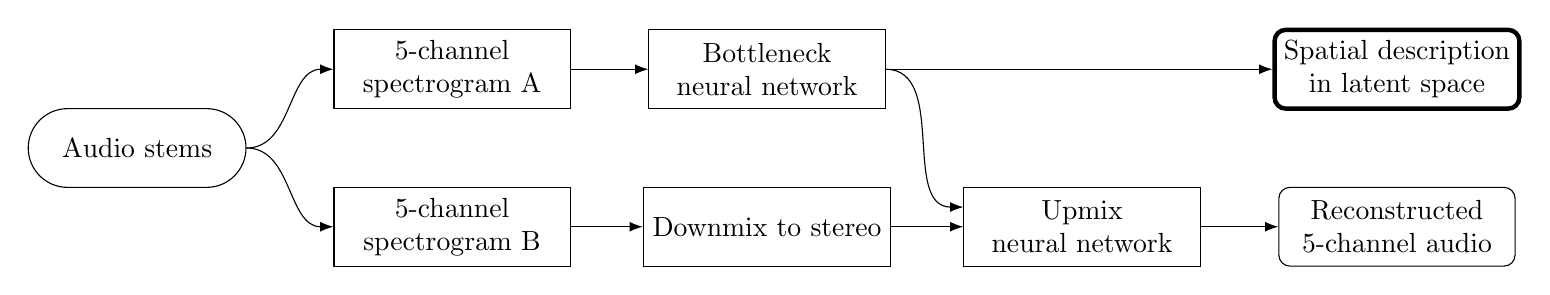
\begin{tikzpicture}[>=latex, node distance=4cm]

        \node[flow_input] (stems) {Audio stems};
        \node[flow_process] (audio5r) [right of=stems,yshift=1cm] {5-channel\\spectrogram A};
        \node[flow_process] (audio5a) [below of=audio5r,yshift=2cm] {5-channel\\spectrogram B};
        \node[flow_process] (bottleneck) [right of=audio5r] {Bottleneck\\neural network};
        \node[flow_process] (downmix) [right of=audio5a] {Downmix to stereo};
        \node[flow_process] (upmix) [right of=downmix] {Upmix\\neural network};
        \node[flow_output,ultra thick] (latentvec) [right of=bottleneck,xshift=4cm] {Spatial description\\in latent space};
        \node[flow_output] (recon) [right of=upmix] {Reconstructed\\5-channel audio};

        \draw[arrow] (stems) to [out=0,in=180] (audio5r);
        \draw[arrow] (stems) to [out=0,in=180] (audio5a);
        \draw[arrow] (audio5r) to [out=0,in=180] (bottleneck);
        \draw[arrow] (audio5a) to [out=0,in=180] (downmix);

        \draw[arrow] (downmix) to [out=0,in=180] (upmix);
        \draw[arrow] (bottleneck) to [out=0,in=180] ([yshift=0.25cm]upmix.west);
        \draw[arrow] (upmix) to [out=0,in=180] (recon);
        \draw[arrow] (bottleneck) to [out=0,in=180] (latentvec);
        
        \end{tikzpicture}
    }
    \caption{Architecture digram of \citeauthor{yangUpmixingStyleTransfer2022}'s neural network that learns a spatial representation of its audio training data. The latent vector (shown in a thick outline) can be used as a description of the spatial image. Spectrograms A and B use the same stems but different panning parameters. Recreated from \cite{yangUpmixingStyleTransfer2022}.}
    \label{fig:dl_upmix}
\end{figure}

\gls{dl} has also been used outside the music domain to e.g. learn spatial relationships between individual microphones in an array \cite{yangSelfSupervisedLearningSpatial2024}. While such tasks do not directly address the research questions in this thesis, they demonstrate that learning spatial features on large amounts of unlabelled audio data is possible given the appropriate methods and pretext task.

Neural generation of spatial audio also continues to be a hot topic up to the present day, with many attempts to generate high-quality binaural, ambisonic or multichannel audio from mono sources \cite{limEnhancingSpatialAudio2024,liCyclicLearningBinaural2024,liTASPersonalizedTextguided2024,chenCCStereoAudioVisualContextual2025,melechovskySonicMasterControllableAllinOne2025,santosLargeScaleSelfSupervisedLearning2025,wangSpatialV2AVisualGuidedHighfidelity2026}. In doing so, the networks must infer spatial information from a source other than audio (typically an accompanying video or text prompt), and in the process will learn the spatial qualities of their audio training data.

\section{Prediction of perceptual scalars}
\label{sec:prediction_of_perceptual_scalars}
A perceptual scalar is a measurement that would usually be made via a perceptual listening test. \Citeauthor{bergSystematicEvaluationPerceived2003}  give a long list of typical perceptual measures that can be derived from the low-level cues \cite{bergSystematicEvaluationPerceived2003}, although later literature has focused on \gls{asw} and \gls{lev} \cite{rumseySpatialAudioSensory2006}. Those tests are known to be slow and costly \cite{rumseySpatialQualityEvaluation2002}, so prediction of the perceptual scalars via objective means is particularly useful to researchers as it allows for faster experimentation.

\gls{asw} is one of the more common values that has been addressed in the literature. The early work of \citeauthorandnumber{supperOnsetGuidedSpatialAnalyser2005}, \citeauthorandnumber{masonImplementationApplicationBinaural2006}, and \citeauthorandnumber{dewhirstModellingPerceivedSpatial2008} detail the construction of \q{binaural analysers} that are able to estimate \gls{asw}. \citeauthor{dewhirstModellingPerceivedSpatial2008} compares several methods to estimate \gls{asw} given \gls{ild}, \gls{itd}, and \gls{iacc} cues from binaural audio signals. The prediction results were promising, but mixed. \citeauthor{dewhirstModellingPerceivedSpatial2008} even notes that the original values of \gls{asw} given by test participants were somewhat varied, concluding that the test itself was a difficult task.

Since these early experiments the analysis of \gls{asw} has remained a topic of interest, with \citeauthorandnumber{kasbachAssessingContributionBinaural2016}, \citeauthorandnumber{miethObjectiveEvaluationTechniques2017}, and \citeauthorandnumber{antoniukBlindEstimationEnsemble2023} all proposing ways to calculate it. It is not restricted to the binaural domain, with \citeauthorandnumber{sarroffMeasurementsSpaciousnessStereophonic2008}, \citeauthorandnumber{wilsonPerceptionEvaluationAudio2013}, and \citeauthorandnumber{mourgelaExploringTrendsAudio2024} also proposing formulas for generic stereo signals. 

\gls{lev} on the other hand has prompted slightly more varied discussion over the years. An early study by \citeauthorandnumber{soulodreNewObjectiveMeasures2004} compared several objective measures for it. The methodology was to fit a correlational model that predicted the output of perceptual test from objective audio measures. The objective measures were based on either the \gls{iacc} or \gls{lef} of the audio signal. \citeauthor{soulodreNewObjectiveMeasures2004} notes that the late-arriving sound ($>80$ms after the sound's onset) are most relevant to \gls{lev}, regardless of which objective measure is used. \citeauthorandnumber{sunishDevelopmentValidationUnintrusive2010}, \citeauthorandnumber{powerInvestigationImpact3D2013}, \citeauthorandnumber{jacksonEstimatesPerceivedSpatial2010}, and \citeauthorandnumber{nowakPerceptionPredictionApparent2017} later expanded the same concept by fitting models on different objective audio measures. 

\citeauthor{dewhirstObjectiveAssessmentSpatial2005} propose a different measure in \cite{dewhirstObjectiveAssessmentSpatial2005} which involves calculating the area covered by the plurality of individual sound sources after estimating their directional localization. Although, by the authors' own admission, this is a crude measure and was not validated by perceptual tests.

Notably, the prediction of \gls{lev} appears to be used more often to assess spatial audio reproduction (sometimes rendered to binaural), rather than plain stereo. \citeauthorandnumber{powerInvestigationImpact3D2013} even include both mono and stereo reproduction in their experiment, concluding that their subjective ratings for \gls{lev} were considerably lower than all spatial formats. \citeauthorandnumber{sunishDevelopmentValidationUnintrusive2010} also state that \gls{lev} might not be cleanly separable from \gls{asw}.

Within the context of this thesis, the absolute accuracy of any prediction is not necessarily of primary importance. Rather, it matters that the value calculated for each recording in a corpus provides suitable comparisons to the other recordings. \citeauthor{mourgelaExploringTrendsAudio2024}'s work on trends in music production \cite{mourgelaExploringTrendsAudio2024} is one example of such a study. The study groups raw stereo width calculations into 4 buckets, thereby showing that finding recordings with similar stereo width is of more interest than the absolute value.


\section{Spatial quality comparison}

The \glspl{sip} described in \cref{sec:spatial_cues,sec:stereo_image_description,sec:prediction_of_perceptual_scalars} are often used to assess the spatial degradation of an audio signal after some sort of distortion has been applied. A typical method is to calculate the same spatial descriptor on both a reference and degraded signal, then calculate the difference in those descriptors. There is sometimes an additional aggregation step to reduce a multidimensional descriptor down to a scalar.

The types of distortion vary, although a major industrial use is in the development of lossy codecs. The work of \citeauthorandnumber{youSpatialLocalizationEvaluation2012}, \citeauthorandnumber{wangObjectiveMeasurementSpatial2015}, \citeauthorandnumber{delgadoObjectiveMeasurementStereophonic2019}, and \citeauthorandnumber{delgadoObjectiveAssessmentSpatial2019} do exactly this. \Cref{fig:spatial_distortion} shows a typical workflow for the measurements of spatial distortion used in all these studies.

\begin{figure}[htb]
    \centering
    \resizebox{0.618\textwidth}{!}{
        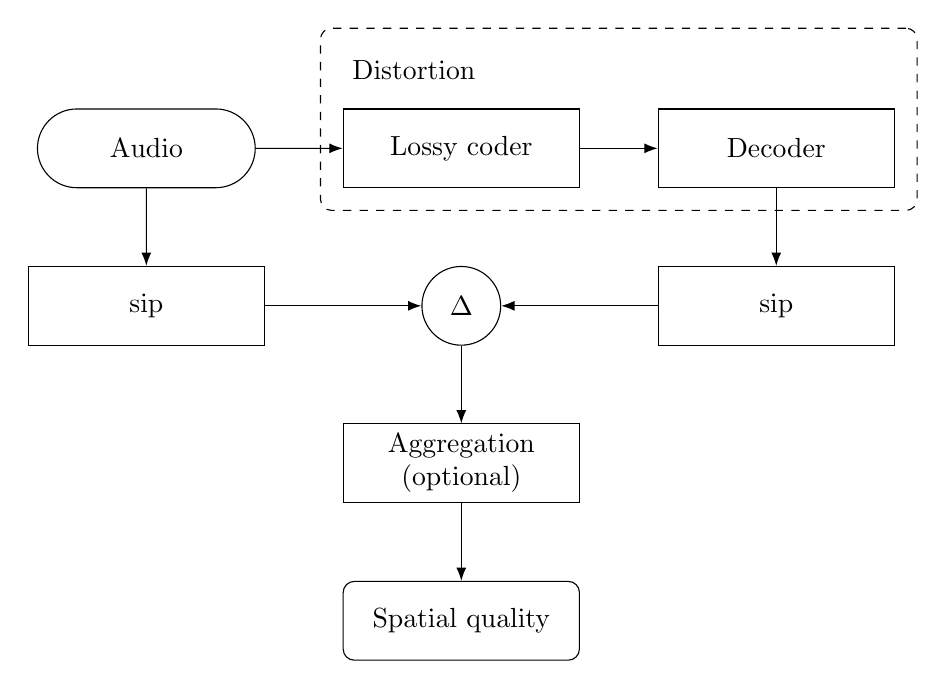
\begin{tikzpicture}[>=latex, node distance=2cm]
            \node[flow_input] (audio) {Audio};
            \node[flow_process] (coder) [right of=audio, xshift=2cm] {Lossy coder};
            \node[flow_process] (decoder) [right of=coder, xshift=2cm] {Decoder};
            \node[flow_process] (sip1) [below of=decoder] {\gls{sip}};
            \node[flow_process] (sip2) [below of=audio] {\gls{sip}};
            \node[draw=black,circle,minimum width=1cm] (diff) [below of=coder] {$\Delta$};
            \node[flow_process] (agg) [below of=diff] {Aggregation\\(optional)};
            \node[flow_output] (dist) [below of=agg] {Spatial quality};

            \node[anchor=west] (dist_label) at ([yshift=1cm]coder.west) {Distortion};
            \node[draw=black,dashed,inner sep=8pt, rounded corners] (distortions) [fit=(coder) (decoder) (dist_label)] {};

            \draw[arrow] (audio) -- (coder);
            \draw[arrow] (audio) -- (sip2);
            \draw[arrow] (coder) -- (decoder);
            \draw[arrow] (decoder) -- (sip1);
            \draw[arrow] (sip1) -- (diff);
            \draw[arrow] (sip2) -- (diff);
            \draw[arrow] (diff) -- (agg);
            \draw[arrow] (agg) -- (dist);
        \end{tikzpicture}
    }
    \caption{Example architecture to measure the spatial quality of a lossy audio codec. The two \gls{sip} blocks must use exactly the same method, although the choice of method is application-specific. The \q{Distortion} block may be replaced when using the workflow for other tasks.}
    \label{fig:spatial_distortion}
\end{figure}

Spatial distortions other than lossy coding have also received attention in more recent years. For example, \citeauthor{barryBinaspectPythonLibrary2025} present a comparison of binaural rendering and downmix algorithms (as well as lossy codecs), showing that minute differences in binaural cues can be easily detected using their methods \cite{barryBinaspectPythonLibrary2025}. Taking the opposite approach, \citeauthor{watcharasupatQuantifyingSpatialAudio2024} demonstrates a new metric for assessing spatial quality and demonstrate it using several common, but artificial distortions \cite{watcharasupatQuantifyingSpatialAudio2024}.

In all the above studies, the detail and implementation of the spatial descriptors vary. Some studies (e.g. \cite{delgadoObjectiveAssessmentSpatial2019,barryBinaspectPythonLibrary2025}) opt to use high-level \glspl{sip} such as \q{directional loudness maps} or \gls{ild} histograms, while others (e.g. \cite{wangObjectiveMeasurementSpatial2015}) use low-level spatial cues such as \gls{ild} and \gls{itd}. In short, both approaches are valid and relevant to the \glspl{rq} presented in this thesis. 

Following from this establishment of objective measurements for spatial quality, it is increasingly common practice to use them as additional terms in \gls{dl} loss functions, thereby allowing the networks to learn spatial features. \citeauthorandnumber{erruzBinauralSourceSeparation2017} demonstrates a loss term based on the \gls{ild} of binaural audio, whereas both \citeauthorandnumber{limEnhancingSpatialAudio2024} and \citeauthorandnumber{giampiccoloModelingImpulseResponse2025} implement an \gls{icld} loss term for various combinations of ambisonic channels. In all these studies, the underlying industry motivation was the generation and rendering of new spatial audio formats, similar to the upmixing research mentioned in \cref{sec:history}.


\section{Analysis of large musical datasets}

Many of the studies cited in \cref{sec:stereo_image_description} use a large dataset of recorded music to demonstrate the effectiveness of their \glspl{sip}. For example, \cite{tzanetakisStereoPanningFeatures2007,tzanetakisStereoPanningInformation2010,tardieuProductionEffectAudio2011} tackle genre recognition, \cite{ziemerAcousticFeaturesRecording2021} predicts artist or \glsxtrshort{dj}, and \cite{tardieuProductionEffectAudio2011} determines the decade of the recordings. Similar studies such as \cite{zhouPredictingGeographicalOrigin2014,kedyteGeographicalOriginPrediction2017} show that the geographic origin of a recording can be determined from audio features, although they don't  include any spatial features. 

\citeauthor{ziemerProducerVsRapper2025}'s continuation of their work on goniometer features (see \cref{sec:stereo_image_description}) uses a dataset comprising songs that were either produced or rapped by specific artists \cite{ziemerProducerVsRapper2025}. They train a \gls{som} on the goniometer features of the dataset. The results firstly show that specific artists have specific sonic profiles, and furthermore that when those artists collaborate, the sound profile of the resulting track is dominated by the producer.

\citeauthor{collinsNewCuratedCorpus2018} collated a dataset of historical electronic music \cite{collinsNewCuratedCorpus2018}. As part of that work, they extracted two spatial metrics: \q{channel loudness difference} and \q{stereo spatial ebb}. The example experiment given to demonstrate the dataset showed that \q{stereo spatial ebb} changes according to the year of the recording, thus indicating an artistic trend over time. \q{Channel  loudness difference}, on the other hand, remained static.

In \citeauthor{panteliCharacterizationSingingStyles2017}'s work on the classification of singing style \cite{panteliCharacterizationSingingStyles2017}, the classes -- instead of being determined by known labels -- are learned by first extracting low-level audio cues, then finding common features within those cues. The features are then used as the input to unsupervised clustering algorithms to determine the relationships of the recordings to each other. \citeauthor{panteliComputationalStudyOutliers2017} continued the work in \cite{panteliComputationalStudyOutliers2017} where outliers in the global dataset where found using similar techniques and links between different musical cultures were drawn. While neither of these studies addressed spatial information, they nevertheless present use cases where unsupervised learning on features extracted from large audio dataset generates cultural knowledge that extends beyond the musical domain. 

On a cautionary note, \citeauthor{chauhanCrossCulturalBiasMelScale2026} recently showed that \gls{ml}-based tasks taking audio input from multiple cultures are biased towards Western sources if they use the Mel spectrogram as the audio frontend \cite{chauhanCrossCulturalBiasMelScale2026}. The authors recommend using alternative frontends, such as \gls{erb}.

What all these studies have in common is an interest in the dataset itself regarding both the relationships between individual recordings, and the relationship of the entire corpus to the wider world. Low-level audio features are of lesser importance, other than to construct the high-level metrics that enable comparison between recordings.

\chapter{Research Methodology}
\label{ch:methodology}
% How do music producers use stereo field?

% RQ1: How does the stereo image of a recording relate to real-
% world musical knowledge?

% RQ2: What methods can be used to describe the stereo image of
% a music recording?

In this chapter I break down the reasoning behind the \glspl{rq} given in \cref{sec:research_questions}, both from philosophical and practical standpoints. I argue that the methods I chose for the research in this thesis allow for a timely and achievable answer to the overarching \gls{rq}.

The overarching \gls{rq} -- \q{How do music producers use stereo field} -- could be approached in many ways. However, the work in this thesis is steeped in the context of large audio datasets. Indeed, the reason for performing the research at the current point in time is the ease of access to said datasets along with the availability of computer processing power to analyse them. From an ontological standpoint this most closely fits the Parmenidean viewpoint of \textit{being}. According to \citeauthor{grayDoingResearchReal2008}, Parmenidean ontology posits that reality is composed of clearly formed entities with identifiable properties \cite{grayDoingResearchReal2008}. If the producers' collective musical output is \q{reality}, then the recordings in the datasets certainly fit that description.

The two smaller \glspl{rq} represent different epistemological perspectives on the overarching one. \rqa{} is based in \textit{constructivism}, where the meaning of the stereo field is imposed on the recordings by the listener. Conversely, \rqb{} is rooted in \textit{objectivism}, where the properties of a recording's stereo field are an objective truth that can be measured. Not only that, but generalizations about the use of stereo field across the entire population of recordings are also objective and measurable. While the two epistemologies are somewhat adverse to each other, they both fall under the ontology of \textit{being} \cite{chiaProductionManagementKnowledge2002}.

Under \textit{constructivism}, one valid research methodology is \q{heuristic inquiry} -- the act of totally immersing oneself in the phenomenon being researched and allowing intuition to guide the understanding of the \gls{rq}. I used this technique for a sizeable part of the work described in this thesis. For example, {paper~\ref{paper:auxtrument}} is a retrospective account of building a new musical instrument where the primary sonic material was the signal from a remote stereo microphone. The act of building the instrument, listening to its output, and forming ideas about which sonic phenomena were interesting was a direct way to relate the stereo field with musical knowledge, addressing \rqa{}. While this provides a basis for other research, critics of heuristic inquiry will point out that it is deeply personal and therefore not particularly generalizable \cite{grayDoingResearchReal2008}.

To complement the \textit{constructive} approach and form more robust conclusions about an entire population of music producers, I concurrently embarked on a more objective research path. The epistemology of \textit{operationalism} is defined by the principle that in order to understand something, it must be measurable \cite{changOperationalism2021}. Thus, to understand stereo field, a set of operations to measure it is necessary. In practice, that means a software library capable of analysing music recordings and extracting information about their stereo field. The benefits of creating this software are threefold. Firstly, it enables comparative measurements of disparate music recordings, allowing one to validate and challenge the existing research described in \cref{sec:related_works}. Secondly, the methods used for any experimental research must be controllable and repeatable. A software library is a fantastic way to achieve this. Thirdly, the act of writing the library can be seen as a similar act of immersion to that previously described in the \textit{constructive} research. By breaking down the measurement of stereo field into simple instructions, one is forced to think about quantifiable relationships between audio phenomena. \citeauthor{wiltschkoLanguageThoughtCommunication2022} argues that language is a tool for both thought and communication in equal measure \cite{wiltschkoLanguageThoughtCommunication2022}. It follows that computer code (which is a written language like any other) acts as both a representation of the creator's thought process, and the communication of those thoughts to any readers. The software written for this thesis was therefore fundamental to the research process, as well as underpinning the results of paper \ref{paper:dafx}.

This combinatorial approach is not a new idea. The 13th century philosopher Nicolaus Cusanus spoke about two foundations of knowledge - \q{ratio} (that which you measure) and \q{intellectus} (the relationship to the unknown) \cite{millerCusanusNicolausNicolas2025}.  It captures the dichotomy that when measuring a phenomenon, more measurements will give one a more accurate picture of the truth, but one must have the forethought to imagine that the measurements might not be able to represent the entire truth. Cusanus argued that both are necessary to make sense of the world, and modern academics propose that as our world is increasingly measured and rationalized, intellectus becomes increasingly important \cite{hylvingRatioIntellectusConceptual2022}.

One potential criticism of this combinatorial approach is that an answer to the overarching \gls{rq} could instead be gained by gathering interview or observational data (using \citeauthor{yinCaseStudyResearch2014}'s taxonomy of \q{evidence sources} \cite{yinCaseStudyResearch2014}).  As \citeauthor{grayDoingResearchReal2008}'s assessment of the strengths and weaknesses of each evidence type states \cite{grayDoingResearchReal2008}, the former (interviews and observation) result in deep, contextually rich data, but are time-consuming to collect and subject to biases from the act of interviewing or observing itself. More specific to the music community, there is an inherent understanding that music is a form of language \cite{agawuMusicDiscourseSemiotic2014}. Adding a layer of indirection (interviews conducted in spoken language) only serves to muddy the resulting data. Indeed, \citeauthor{hospersConceptArtisticExpression1954} argues that an artist's expression is inherently intertwined with the creation the original art form, noting that the intentions are sometimes so complex and multifaceted as to defy explanation even to the artist themselves \cite{hospersConceptArtisticExpression1954}. In contrast, the musical datasets that we are presented with would be classified as \q{archival records} or \q{physical artefacts}, which according to \citeauthor{grayDoingResearchReal2008} are precise and technically insightful, but prone to selectivity and reporting biases \cite{grayDoingResearchReal2008}. 

I argue in this thesis that such biases can be partially mitigated by combining research from multiple epistemologies. While \textit{objective} research can determine what music producers do from a technical perspective, \textit{constructive} research can offer insight into the choices and trade-offs they made to end up at their final artistic output. The work I have performed for this thesis is a combination of immersion in musical practice, thorough reviews of existing literature, and detailed implementation of audio \gls{dsp} analysis techniques. This combination presents a well-rounded viewpoint on the original \glspl{rq}, as well as giving rise to new questions that could be answered in the continuation to doctoral studies (see \cref{sec:future_work}).

\chapter{Paper summaries}
\label{sec:paper_summaries}

\section*{Paper \ref{paper:auxtrument}}

\textbf{\citetitle{franklinDevelopmentWebBasedRealTime2025}}

\subsection*{Authors}
\citefullauthors{franklinDevelopmentWebBasedRealTime2025}

\subsection*{Status}
Published in \citepublication{franklinDevelopmentWebBasedRealTime2025}, \citedate{franklinDevelopmentWebBasedRealTime2025} \cite{franklinDevelopmentWebBasedRealTime2025}.

\subsection*{Research methods}
This paper presents a retrospective of a project to build a distributed audio performance over mobile networks. It follows the practice-based research methodology as defined by \citeauthorandnumber{candyPracticeBasedResearch2006}.

\subsection*{Results and conclusions}
The paper documents a real use case where stereo field and reproduction thereof is of prime importance. One conclusion was that network reliability was a limiting factor of the audio performance, sometimes leading to a degraded spatial impression. Research question \ref{rq:usecase} is addressed -- Finding an adequate balance between audio spatial quality and network utilization would require tools to measure the stereo image.

\subsection*{My contribution}
Member of the team that conceptualized the Auxtrument and made the initial survey and prototyping of existing audio transmission technologies. Responsible for post-prototyping of alternative approaches and custom audio software.

\clearpage
\section*{Paper \ref{paper:slr}}
\textbf{\citetitle{miticSystematicLiteratureReview2026}}

\subsubsection*{Authors}
\citefullauthors{miticSystematicLiteratureReview2026}

\subsubsection*{Status}
Accepted to \citepublication{miticSystematicLiteratureReview2026}, May 2026

\subsubsection*{Research methods}
\gls{slr} following the \gls{prisma} standard to gather all currently available methods for determining spatial features of stereophonic musical audio.

\subsubsection*{Results and conclusions}
Addressing \rqb{}, the review revealed a comprehensive set of techniques that can be used to make spatial descriptions of stereo music, encompassing low-level spatial cues, high-dimensional descriptors, and predictions of important perceptual values. Despite the high number of studies that were assessed, there were relatively few that were \enquote{very relevant} to recorded music specifically. The \gls{slr} also revealed that while \gls{ml}/\gls{dl} have been used on spatial features in the past, both \textit{unsupervised} \gls{ml} and very large music corpora remain fairly unexplored. It also details a framework for how to create a \gls{sip} algorithm that is useful for any given dataset and use case. It acts as a one-stop-shop to springboard any future research into stereo field.

\subsubsection*{My contribution}
Main author, responsible for all data collection and processing, and writing.
\clearpage
\section*{Paper \ref{paper:dafx}}

\textbf{\citetitle{miticObjectiveComparisonPanning2025}}

\subsubsection*{Authors}
\citefullauthors{miticObjectiveComparisonPanning2025}

\subsubsection*{Status}
Published in \citepublication{miticObjectiveComparisonPanning2025}, September 2025

\subsubsection*{Research methods}
Several \gls{dsp} techniques for determining audio spatial features were performed on a small dataset that had predictable musical characteristics. The different techniques were compared using a new objective metric.

\subsubsection*{Results and conclusions}
The paper revealed that although there are several \gls{dsp} techniques specifically designed for the extraction of recording and panning features, they are all limited in their own ways. One particular technique (\gls{spf} from \cite{tzanetakisStereoPanningFeatures2007}) was particularly promising as a candidate for use later in the doctoral phase of studies, and the others could be used with some modifications. Overall it highlighted the importance of choosing both a \gls{sip} and a distance metric that are appropriate to the overarching task, thereby addressing \rqb{}.

\subsubsection*{My contribution}
Main author, responsible for all data collection, experimental design, and software implementation. Presented the paper at the 28th International Conference on Digital Audio Effects in Ancona, Italy.
\clearpage
\section*{Paper \ref{paper:bth}}
\textbf{\citetitle{miticPerceptualEvaluationBinaurally2026}}

\subsubsection*{Authors}
\citefullauthors{miticPerceptualEvaluationBinaurally2026}

\subsubsection*{Status}
In review at \citepublication{miticPerceptualEvaluationBinaurally2026}, August 2026. 

\subsubsection*{Research methods}
A perceptual test was used to determine listeners' reactions to carefully constructed audio stimuli. Standard statistical analysis was performed on the raw test results.

\subsubsection*{Remaining Work}
Await peer review and address any comments.

\subsubsection*{Results and conclusions}
The paper concluded that when listeners are presented with voice overlaid on top of music, the best panning position for the voice was not always in the default centre position. The data showed that test participants held strong individual preferences regarding which panning position sounded best, although the demographic data collected on them did not explain their preferences. Counterintuitively, the data did not reveal any link between the music track and the preferred panning position. We speculated that performing a much wider study using more music tracks with more controlled vocal elements might reveal more.

\subsubsection*{My contribution}
Joint main author alongside Majed Elwardy. Contributed to experiment design, data analysis, software implementation, and writing.
\chapter{Discussion}
\label{ch:discussion}

As mentioned in \cref{ch:methodology}, the work listed in this thesis happened in the context of easy access to vast music datasets. This access certainly influenced both the methods I used for each paper, and the research questions themselves. One can envision a quasi-mirror-image research process where instead of beginning with a research question and collecting data to find an answer, one must ask \mbox{\textit{\q{what knowledge can I pull from the available data?}}}. 

It was precisely this setting that made the combinatorial philosophical approach detailed in \cref{ch:methodology} so suitable. By immersing myself in the world of stereo image, the research questions germinated, evolved, and eventually coalesced into their current form. The need to consider what kind of knowledge was hiding in the data spurred a downstream need to understand what musical knowledge the producers and musicians could have imparted via their creative process. \rqa{} was the outcome of that thinking. By contrast, \rqb{} was a relatively straightforward concoction once \rqa{} started to materialize. One could even consider \rqb{} to be part of the answer to \rqa.


The fact that I focused on stereo image was somewhat of a practical choice. Firstly, it had a handful existing industrial use cases but potential for more. Secondly it was relatively under-studied in previous literature - certainly not at the scale that is possible today.

With that said, we must now address the proverbial elephant in the room. Despite what one might imagine from the title of this thesis, the included papers do not deal with \q{vast repositories of recorded music} directly. Rather, they all focus on understanding what is possible to find in those datasets, and subsequently how to find it. I do not consider this a contradiction in terms, but rather an optimistic indication that answers to the two minor \glspl{rq} contribute to answering the overarching \gls{rq} as well as exposing new knowledge gaps that require more research.

Previous research into stereo field generally followed a simple pattern: A novel algorithm is proposed, calculated on a mid-size music collection, and then used to predict labels that were known a-prori. The gap I identified was a lack of understanding into what musical features the existing algorithms have the ability to recognize. Once that is established, it would be possible to examine the available datasets with the intention to understand how a huge population of creatives choose to express themselves though their music. That research will reveal the scale and variation of stereo techniques that musicians are able to employ in their work. Given the basic knowledge gained from the work in this thesis, it might then be possible to reason about how musicians and producers sculpt their stereo fields, relating it both to the musical content and the wider context in which it was created.


\section{Future work}
\label{sec:future_work}

The work documented in this licentiate thesis provides the theoretical and practical basis for analysis of stereo image in music recordings. The focus was on amassing the signal processing techniques that enable the analysis of stereo field, and testing their applicability to various types of recordings that were known a-priori. The next stage of research will involve applying the knowledge from this thesis on much larger musical corpora. The signal processing techniques will be honed and run on vast musical datasets, secure in the knowledge that they will generate data appropriate to the experiment at hand.

During the licentiate, several points arose that provoked further investigation. Firstly, the available public datasets of recorded music are generally encoded using lossy compression. While lossy compression algorithms undergo perceptual tests in their development, it is unclear how they affect spatial cues at the scale of said datasets (which encompass much musical variation). The spatial effects of lossy compression therefore warrant further investigation. Secondly, the public datasets are generally formed from online services where musicians have uploaded their own recordings for free. In contrast, professional recordings (which are much more numerous) are not included in any public datasets. Since professional recordings make up the vast majority of recorded music, it needs to be assessed whether public datasets are representative of professional recordings.

In short, the doctoral research will tackle a larger problem of assessing human musical creativity though the recorded output. The techniques surfaced by the licentiate will provide the foundation, and will be applied to real-world data.


\begin{appendices}

\chapter{Demonstration Audio Files}
\label{app:demo_tracks}

\section*{Demo tracks}

These tracks from the \gls{fma} dataset \cite{defferrardFMADatasetMusic2017} were used to generate diagrams of spatial cues and \glspl{sip} in \cref{sec:related_works}.

\bigskip 
% \resizebox{0.94\columnwidth}{!}

{
    \footnotesize
    \begin{tabular}{rllll}
\toprule
Track ID & Artist & Title & Genres & Letter \\
\midrule
123899 & Rachel Mason & Rebel Angels & Singer-Songwriter & A \\
117614 & Blue Dot Sessions & Red City Theme & Soundtrack, Instrumental & B \\
122809 & The Carnys & foolsgame & Experimental Pop & C \\
\bottomrule
\end{tabular}

}


\section*{Freesound files}

These sound clips from \href{https://freesound.org}{Freesound} \cite{Freesound} were used to generate diagrams in \cref{ch:background}.

\bigskip 

{
    \footnotesize
    \begin{tabular}{rll}
\toprule
Sound ID & Name & URL \\
\midrule
581451 & kick & \url{https://freesound.org/people/johnnydekk/sounds/581451} \\
581473 & hihat & \url{https://freesound.org/people/johnnydekk/sounds/581473} \\
31912 & speech & \url{https://freesound.org/people/acclivity/sounds/31912} \\
\bottomrule
\end{tabular}

}

% \section*{Miscellaneous}

% The recording of anechoic singing used in the \gls{daw} session shown in \cref{fig:daw} was downloaded from \url{https://www.angelofarina.it/Public/Anecoic/nontam48.wav}.

\end{appendices}

\printglossaries

\printbibliography

\clearpage  % Forces BibTeX to process the entire document

\end{document}